\begin{quotation}
  {\footnotesize
    \noindent{\emph{``Prediction is very difficult, especially if it's about the future.''\\}
    }
    \begin{flushright}
      Niels Bohr
    \end{flushright}
  }
\end{quotation}
\vspace{0.5cm}

Performing a robust pose initialization from a \acrshort{2d} image captured by a monocular camera in space is a very though task, particularly due to the fact that illumination conditions in space may vary during a single orbit, and therefore may cause inaccurate and unreliable features detection. Moreover, the Earth presence in the background introduces a major complexity into distinguishing the target \acrshort{sc} shape from the Earth surface. The \acrshort{svd} pose initialization architecture aims at solving the problem of pose initialization by employing a single \acrshort{2d} image taken by a monocular camera. In this chapter, a detailed description of the \acrshort{svd} architecture implementation which has been carried out in this work is presented.

\section{Feature-Based Pose Estimation}
The images generated  trough the toolbox presented in Chapter~\ref{chap:second-chapter} are here analyzed using the robust monocular vision-based pose initialization algorithm proposed by S. Sharma, J. Ventura and S. D'Amico in \cite{Sharma2018}.
The problem of pose initialization consists in computing the rotation matrix,\gls{A_TC} and the translation vector, \gls{t_c} that describes the transformation between the camera frame, $C$, and the target body frame, $B$. Given a generic image point, $\mathbf{p}$ = $ [u, \ v]^T $, it is possible to relate the $\mathbf{q_B}$ point of the \acrshort{3d} model with the corresponding $\mathbf{r_C}$ point in camera coordinates by employing the standard pinhole camera model (the interested reader can found a brief introduction to the pinhole camera model in Appendix~\ref{subsection:pinhole}):

\begin{equation}
  \mathbf{r_C} = \left[x_C \quad  y_C \quad z_C\right]^T = \mathbf{A_{TC}} \; \mathbf{q_B} + \mathbf{t_C} \,,
  \label{eq:rc}
\end{equation}

\begin{equation}
  \mathbf{p} = \left[ \frac{x_C}{z_C} f_x + C_x , \ \frac{y_C}{z_C} f_y + C_y \right] \,,
  \label{eq:p}
\end{equation}

where \gls{fx} and \gls{fy} are the respectively the horizontal and the vertical focal length and $ \left[C_x, \ C_y \right]$ are the coordinates of the center of the image. Moreover, it is assumed - without loss of generality - that the direction $\mathit{C_3}$ of the camera frame is pointed along the boresight of the camera and the directions $\mathit{C_1}$ and $\mathit{C_2}$ are aligned with the image frame defined by $P = \left( \mathit{P_1}, \ \mathit{P_2} \right)$.

\begin{figure}[htbp]
  \centering
  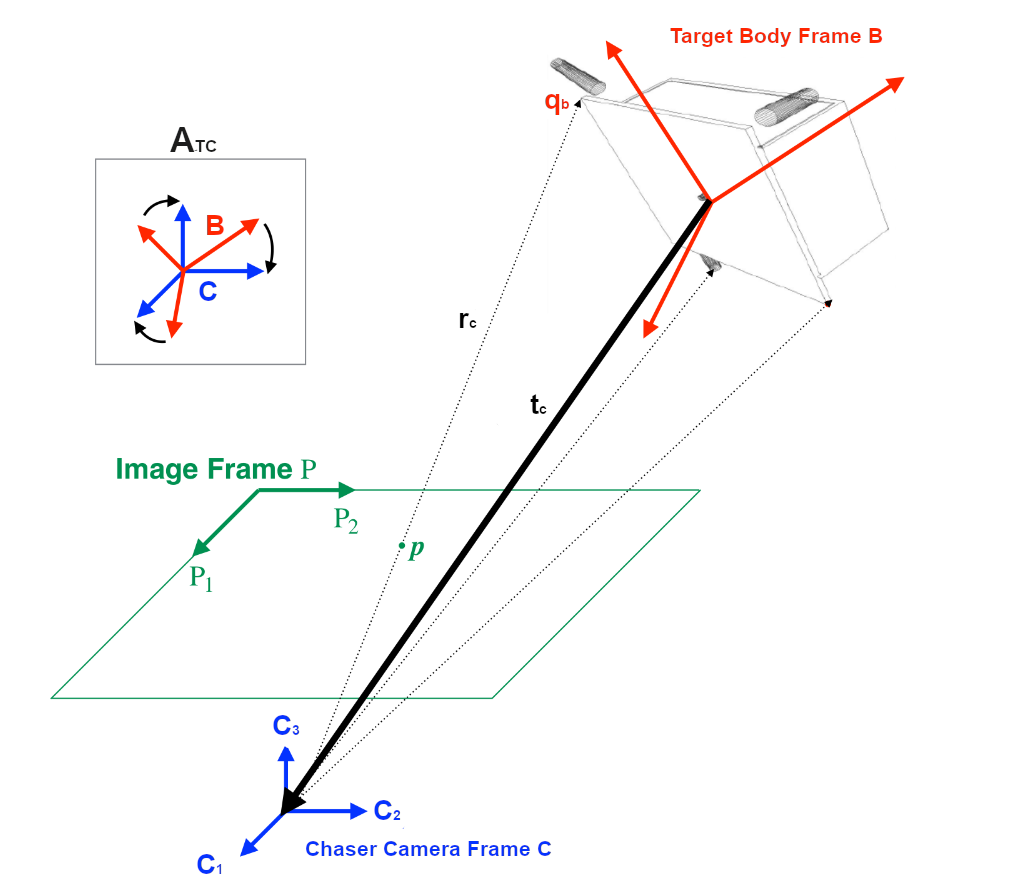
\includegraphics[width=0.72\textwidth]{gfx/poseProblem.eps}
  \caption{Schematic representation of the pose estimation problem using a monocular image \cite{Sharma2018}.}
  \label{fig:theposeproblem}
\end{figure}

As discussed in \cite{D2014}, it is possible to build several considerations on top of those two coupled equations:

\begin{itemize}
  \item the relationship between image points and pose parameter is hightly non linear and the problem of retrieving the \acrshort{3d} points from the \acrshort{2d} image can have infinite solution in under-constrained situations \cite{10.1145/358669.358692};
  \item there is no \textit{a priori} knowledge of the correspondence between $\mathbf{q_B}$ and $\mathbf{p}$;
  \item the image coordinates need to be corrected for pixel's non-quadratism and lens distortion before using the perspective projection equations.
\end{itemize}

The pose estimation system thus needs the capability of extracting the client features from the available image (image processing) to obtain measurements, namely  $\mathbf{p}$. The extracted features then needs to be matched to the correspondent elements of a client model (model matching), namely $\mathbf{q_B}$. The unknown pose then has to be estimated based on the available measurements (pose estimation).
To be able to uniquely solve Equations \eqref{eq:rc} and \eqref{eq:p}, at least six correspondences between the image points and the model points are needed. \cite{10.1145/358669.358692}. The challenging part of the problem is to be able to correctly detect the most meaningful points in the \acrshort{2d} image. Usually this can be achieved by employing edge detection techniques, such as the Canny edge detector \cite{10.1109/TPAMI.1986.4767851} followed by the Hough transform \cite{10.1145/361237.361242}. This approach however may be biased if applied directly to the image due to the fact that these algorithm are gradient based and are not able to correctly distinguish the foreground from the background and also requires the definition of numerous hyper-parameters which are difficult to tune for broad applicability because the imaged scene and the illumination conditions are constantly changing throughout the orbit \cite{Sharma2018}.

\subsection{General Architecture}
The architecture proposed in \cite{Sharma2018} tries to solve the pose estimation problem by:

\begin{itemize}
  \item coupling the \acrfull{wge} technique with the Sobel edge detection to perform the image processing;
  \item using feature synthesis to reduce the search space for model matching;
  \item combining a \acrshort{pnp} solver with the \acrfull{nr} method for pose estimation.
\end{itemize}

\begin{figure}[htbp]
  \centering
  \includegraphics[width=1.0\textwidth]{gfx/SVDPipeline.eps}
  \caption{The \acrshort{svd} architecture for solving the pose estimation problem \cite{Sharma2018}.}
  \label{fig:svdArchitecture}
\end{figure}

As the reader can see from the schematic represented in Figure~\ref{fig:svdArchitecture}, the pipeline is composed from two different subsystems:
\begin{itemize}
  \item the image processing subsystem, which receive as an input a \acrshort{2d} image, distinguishing the \acrshort{sc} from the image, extract its edge features and groups them into geometric groups;
  \item the pose determination subsystems, which acceps as input the previously feature groups detected by the image processing subsystem and the \acrshort{3d} model. It then pairs the \acrshort{2d} and \acrshort{3d} geometric groups to formulate multiple correspondence hypotesis. For each hypothesis formulated, the endpoints of the line segments forming the geometric groups are used to solve Equation \eqref{eq:rc} and Equation \eqref{eq:p}. The five best solution then are iteratively refined by employing the \acrshort{nr} method.
\end{itemize}

Two are the most meaningful innovation the \acrshort{svd} architecture introduces:
\begin{itemize}
  \item the usage of the \acrshort{wge} technique in order to distinguish the target \acrshort{sc} from the background and for enhancing the output of the edge detection procedure bu providing a robust identification of the small as well as large edges of the \acrshort{sc};
  \item the usage of feature groups detected in the image and in the \acrshort{3d} model to solve the feature correspondence problem, which also allows the \acrshort{svd} architecture to be more computationally efficient.
\end{itemize}

\subsection{Image Processing Subsystem}
The taks of the image processing subsystem is to extract the most meaningful features from the \acrshort{2d} image a of the target \acrshort{sc}. To effectively and rapidly detect the target \acrshort{sc} edges - even in presence of the Earth in the background - an hybrid image processing subsystem is proposed in \cite{Sharma2018}.
By fusing together the \acrshort{wge} technique and classical state-of-the-art edge detection techniques the architecture proposed by Sharma \textit{et al.} is capable to provide a robust and efficient identification of the true edges of the \acrshort{sc}.
In particular, the \acrshort{wge} technique is able to identify a \acrfull{roi} in a more accurate and robust way with respect to state-of-art techniques. The \acrshort{roi} detection not only makes the entire subsystem robust against the background, but also allows an automated selection of the hyper-parameters needed for the Hough transform, which is used to detect both small and large features of the \acrshort{sc}, in contrast with state-of-the-art algorithms which rely on a single set of manually tuned hyper-parameters.
The flow of the image processing subsystem is illustrated in Figure~\ref{fig:imageProcessingSubsystem}.

\begin{figure}[htbp]
  \centering
  \includegraphics[width=1.0\textwidth]{gfx/imageProcessingSubsystem.eps}
  \caption{The image processing subsystem \cite{Sharma2018}.}
  \label{fig:imageProcessingSubsystem}
\end{figure}

\subsubsection{\acrshort{roi} Detection}
The first thing to perform when analyzing an image is to identify a \acrshort{roi}.
The raw input image, assumed to be rectified (\textit{i.e.},
corrected for lens distortion), is firstly imported in MATLAB. After that, A Gaussian filter is applied in order to the decrease the magnitude of image noise. The Gaussian filtering can be carried out by using the MATLAB function \textbf{imgaussfilt}. In this work, the images generated with the toolbox presented in Chapter~\ref{chap:second-chapter} are filtered by using a standard deviation $\sigma_X = 1.15$ before being fed to the image processing subsystem. During this work, has been observed that the choice of the $\sigma_X$ value is very important for the success of the subsequent steps, as a wrong value can highly impact the effectiveness of the \acrshort{wge} technique. Once the image has been prefiltered, is fed as input to the \acrshort{wge} block, for the computation of the target's \acrshort{roi}. The first step of the \acrshort{wge} technique consist in computing the magnitude of the image gradient, $|\nabla I|$,  using the Prewitt filter to determine the image gradient (for more details about what the image gradient is, refer to Appendix~\ref{sec:imagegradient}).
The \acrshort{sc} can be detected in the image by observing that, under most illumination conditions, in correspondence of the target \acrshort{sc} edges the gradient variation is more pronounced with respect to the background, regardless of the fact that the background is empty or the Earth is behind.
Indeed, to detect the spacecraft, the gradient distribution is normalized using the MATLAB \inlinecode{MATLAB}{mat2gray} function, sorted into $100$ uniformly distributed bins and fitted by and exponential \acrfull{pdf}, described by the equation:

\begin{equation*}
  y = \frac{1}{\mu} e^{-\frac{x}{\mu}} \,.
\end{equation*}

By observing the resulting histogram, it is clearly possible to see that most of the gradient intensities are weak and corresponds to the feature in the background or on the spacecraft surface. The weak gradient pixel locations can be classified by tresholding the \acrshort{pdf} fit to the gradient histogram. The original authors suggest to use a value of $0.99$ to treshold the \acrshort{pdf}, however, for what concerns this work, all the pixel which corresponds to a cumulative distribution inferior to $0.996$ are classified as weak and set to zero instead. Once the weak gradients are set to zero, only the most prominent features of the \acrshort{sc} are present in the image, as shown in Figure~\ref{fig:wgeSteps}.

\begin{figure}[htbp]
  \centering
  \subfloat[Original image.]{\includegraphics[width=0.45\textwidth]{gfx/FeatureDetection/chosenImage.eps}}
  \qquad
  \subfloat[Gradient detection of original image.]{\includegraphics[width=0.45\textwidth]{gfx/FeatureDetection/gradientBeforeTresholding.eps}}
  \qquad
  \subfloat[Histogram of normalized gradient values.]{\includegraphics[width=0.45\textwidth]{gfx/FeatureDetection/gradientDistribution.eps}}
  \qquad
  \subfloat[Output filtered image gradients.]{\includegraphics[width=0.45\textwidth]{gfx/FeatureDetection/imageAfterTresholding.eps}}
  \caption{Different steps of the \acrshort{wge}.}
  \label{fig:wgeSteps}
\end{figure}

By computing the \acrfull{cdf} of the vertical and horizontal gradient of the filtered image obtained by the \acrshort{wge}, it is possible to determine the coordinates of a \acrshort{roi} where the features that yield the strongest intensity variations are located. Then, assuming that the filtered image gradient is normally distributed, the \acrshort{roi} coordinates can be found by limiting each of the previously computed \acrshort{cdf}s between $0.025$ and $0.975$ in order to enclose the central $95\%$ of the normal distribution.

\begin{figure}[htbp]
  \centering
  \includegraphics[width=0.82\textwidth]{gfx/FeatureDetection/ROI.eps}
  \caption{Result of the \acrshort{roi} detection procedure.}
  \label{fig:ROI}
\end{figure}

As noted in \cite{fracchio2019}, for images having a composite background the \acrshort{roi} detection is limited by the presence of interference, so a smarter choice for selecting the bounding box limits is to treshold the \acrshort{cdf}s between $0.005$ and $0.95$. Therefore, only the central $90\%$ of the normal distribution is selected. Restricting the range however negatively affect the \acrshort{roi} detection procedure for images were the background is empty. This problem can be solved by taking into account an additional constant, equal to the $5\%$ of the mean edge length of the \acrshort{roi} for enlarging the \acrshort{roi} boundaries.

\begin{figure}[htbp]
  \centering
  \subfloat[\acrshort{roi} selected by considering only the central $90\%$ of the normal distribution.]{\includegraphics[width=0.47\textwidth]{gfx/FeatureDetection/ROInoConstant.eps}}
  \qquad
  \subfloat[\acrshort{roi} enlarged by adding the $5\%$ of the mean edge length of the previously \acrshort{roi}.]{\includegraphics[width=0.47\textwidth]{gfx/FeatureDetection/enlargedROI.eps}}
  \caption{Improving the \acrshort{roi} detection procedure.}
  \label{fig:roicomparisons}
\end{figure}

One of the innovative features of the \acrshort{wge} technique is that, once the \acrshort{roi} is correctly determined, it is possible to compute a coarse estimation of the the relative position and line of sight even before the pose determination subsystem. By defining the diagonal length of the \acrshort{roi}, $l_{ROI}$, as:

\begin{equation}
  l_{ROI} = \sqrt{{ROI_{width}}^2 + {ROI_{height}}^2} \,,
\end{equation}

a coarse estimation of the range to the target \acrshort{sc} from the origin of the camera frame is given by:

\begin{equation}
  \norm{t_C}_2 = \frac{\nicefrac{((f_x+f_y)}{2}) L_C}{l_{ROI}} \,,
\end{equation}

were \gls{lc} denotes the diagonal characteristic length of the \acrshort{sc} \acrshort{3d} model. By knowing the coordinates of the center of the image, $[C_x, C_y]$ and the coordinates of the \acrshort{roi} center, $[B_x, B_y]$, it is possible to compute the azimuth and elevation angles ($\alpha, \beta$) from the origin of the camera frame, $C$, to the origin of the body-fixed coordinate system, $B$:

\begin{equation}
  \alpha = \arctan{\frac{B_x - C_x}{f_x}} \,,
\end{equation}

\begin{equation}
  \beta = \arctan{\frac{B_y - C_y}{f_y}} \,.
\end{equation}

Once ($\alpha, \beta$) are known, the coarse relative position solution is given by:

\begin{equation}
  t_C
  =
  \begin{bmatrix}
    \cos(\alpha) & 0 & -\sin(\alpha) \\
    0            & 1 & 0             \\
    \sin(\alpha) & 0 & \cos(\alpha)
  \end{bmatrix}
  \begin{bmatrix}
    1 & 0            & 0           \\
    0 & \cos(\beta)  & \sin(\beta) \\
    0 & -\sin(\beta) & \cos(\beta)
  \end{bmatrix}
  \begin{bmatrix}
    0            \\
    0            \\
    \norm{t_C}_2
  \end{bmatrix} \,.
\end{equation}

As a side note, the coarse pose estimation may be negatively affected if the ratio between the shortest dimension and the longest dimension of the target is high. In fact, in such peculiar case, depending on the target attitude in the particular image that is being processed, the target's apparent dimension may be highly different with respect to its true dimension.

\begin{figure}[htbp]
  \centering
  \includegraphics[width=0.65\textwidth]{gfx/coarsePoseEstimation.eps}
  \caption{Calculation of a coarse relative position solution using the WGE technique \cite{Sharma2018}.}
  \label{fig:coarseRelative}
\end{figure}

\subsubsection{Feature Detection}\label{sec:featureextraction}
The aim of the feature detection block is to  identify and extract from the input image a set of segments that corresponds to the true edges of the target \acrshort{sc} trough the usage of the Hough transform. When applied to the problem of detecting straight lines into an image, the Hough transform performs a shape identification through a voting procedure in the parameter space ($\rho$, $\theta$) (for more details about how the Hough transform work, the interested reader can refer to Appendix~\ref{sec:hough}). Computing the Hough transform using MATLAB, requires the definition of some parameters, which for instance are:

\begin{itemize}
  \item the desired resolution of $\rho$ and $\theta$,
  \item the maximum number of peaks to identify in the Hough transform matrix,
  \item the expected minimum length of the the line segment, \gls{l_min},
  \item the expected minimum length of the the line segment, \gls{lambda} and the maximum gap between two points to be considered in the same line segment, \gls{lambda}.
\end{itemize}

The geometrical constraints imposed to the Hough transform are dictated by the choice of \gls{l_min} and \gls{lambda}, which are usually called hyper-parameters in the \acrshort{cv} field. As can be seen from Figure \ref{fig:imageProcessingSubsystem}, two different streams of features are extracted by means of the Hough transform.\\
%\paragraph{Stream 1: \acrshort{wge}}
The first stream comes from the application of the Hough transform to the full \acrshort{wge} filtered image. Fixing a value of (\gls{l_min}, \gls{lambda}) for all the images will result into the inability of the algorithm to adapt to different distances between the camera and the target. In fact, as the camera moves closer and closer to the target, the latter will fill larger and larger portions of the image, and the expected lengths of its edges in the image plane are expected to grow, so a recomputation of the geometrical hyper-parameters would be needed. However, it is reasonable to hypothesize that the size of the detected \acrshort{roi} bounding box will grow too, so, in \cite{Sharma2018} is proposed to scale the geometrical hyper-parameters by using the information about the \acrshort{roi} diagonal length:

\begin{equation*}
  L_{min,Hough} = \kappa_1 l_{ROI} \ \ \ \  \lambda_{Hough} = \kappa_2 l_{ROI}  \,,
\end{equation*}

were $\kappa_1$ and $\kappa_2$ are two scalars constants which can be empirically tuned off-line.\\

%\paragraph{Stream 2: \acrfull{seh}}
To obtain the second stream of features, first the Sobel operator is applied to the full unfiltered, rectified image, using the MATLAB function \textbf{edge} (for more details about what the Sobel operator is, refer to Appendix~\ref{sec:imagegradient}) . The Sobel operator is applied by imposing an intensity treshold equal to $0.04$. As proposed in \cite{fracchio2019}, in order to eliminate the pixel chunks belonging to smaller reflective elements from the output of \textbf{edge}, it is possible to filter the output by using the MATLAB function \textbf{bwareaopen} which, once minimum pixel number $P$ is defined, it removes all connected components (objects) that have fewer than $P$ pixels from the input binary image. In contrast with what done in \cite{fracchio2019}, which sets $P = 10$ for all images, in this work the $P$ value is computed adaptively for each image, exploiting the information about the \acrshort{roi} diagonal length:

\begin{equation*}
  P = \lfloor \eta \ l_{ROI}
\end{equation*}

where $\lfloor$ is the commonly used symbol for the \inlinecode{MATLAB}{floor} operator and $\eta$ is a multiplicative constants which can be tuned empirically. After that, the Hough transform is applied on the output produced by \inlinecode{MATLAB}{bwareaopen} in order to extract line segments corresponding to the silhouette of the large components of the target. For computing the \acrfull{seh} stream of features, in \cite{Sharma2018} is advised to scale the geometrical hyper-parameters needed to compute the Hough lines by using the information about the \acrshort{roi} diagonal length:

\begin{equation*}
  L_{min,Hough} = \kappa_3 l_{ROI} \ \ \ \  \lambda_{Hough} = \kappa_4 l_{ROI}  \,,
\end{equation*}

where again, $\kappa_3$ and $\kappa_4$  are two multiplicative constants which can be empirically tuned off-line. When the Hough transform is applied to the image processed trough the Sobel operator, it can happen that the output may contain spurious edges, not belonging to the target. For example, this could be the case if a composite background is present in the image. The knowledge the \acrshort{roi} location, obtained through the \acrshort{wge} technique, can now be exploited to \textit{a posteriori} reject any line segment belonging to the \acrshort{seh} stream for which the midpoint lies outside the \acrshort{roi} itself. Do note that this additional step is not needed on the first stream, the one which comes from the application of the Hough transform to the \acrshort{wge} filtered image, because the \acrshort{wge} filters out all the background noise by design.

To set the parameters $\kappa_1$, $\kappa_2$, $\kappa_3$ and $\kappa_4$ several strategies can be followed. For example, the idea proposed in \cite{Sharma2018} is to tune the values of $\kappa_1$ and $\kappa_2$ in order to only extract short line segments from the output of the \acrshort{wge}, and tune the values of $\kappa_3$ and $\kappa_4$ in order to extract large line segments from the output of the Sobel filter. In \cite{fracchio2019} instead is proposed to set similar hyper-parameters for the two stream to achieve some sort of redundancy. In this work, the strategy adopted was to obtain a mix between those two behaviors. \\
To ease the writing of the following sections, from here on the streams of features obtained from the application of the Hough trasform to the \acrshort{wge} filtered image are referred as simply "\acrshort{wge} stream", while the streams of features obtained by the application of the Hough transform on the image processed trough the Sobel operator and the \inlinecode{MATLAB}{bwareaopen} function are simply referred as "\acrshort{seh} stream".

\subsubsection{Merging Edges}\label{sec:mergingedges}
The output of the Hough transform may results in multiple truncated edges, especially when applied to the images processed by the \acrshort{wge} technique. Since fragmentation can increase both the uncertainty and the computational cost of the feature matching and pose solving procedures \cite{fracchio2019}, a section of the \acrshort{svd} architecture is dedicated to find and merge line segments which may corresponds to the same true line segment into a single line segment. The original authors \cite{Sharma2018} perform this step only on the \acrshort{wge} stream. For what concerns this work, to enhance robustness of the whole architecture, it has been decided to apply this step to both the streams.
To check whether two line segments can be considered similar and merged into one single edge, it is possible to define some geometrical checks on the basis of the parameters $\rho$ and $\theta$.
With reference to Figure~\ref{fig:rhotheta}, which shows the polar representation of a straight line in the image coordinate system\footnote{The image coordinate system is characterized from having the positive x axis pointing to the right, the positive y axis pointing downward and the positive z axis pointing toward the direction given by $  \mathbf{\hat{z}} = \frac{\mathbf{\hat{x}} \wedge \mathbf{\hat{y}}}{\norm{\mathbf{\hat{x}} \wedge \mathbf{\hat{y}}}}$.}, $\rho$ represents the distance from the origin to the line along a vector perpendicular to the line itself, while $\theta$ represents the angle of the perpendicular projection from the origin to the line measured in degrees clockwise from the positive x-axis.

\begin{figure}[htbp]
  \centering
  \includegraphics[width=0.45\textwidth]{gfx/hough_rho_theta_diagram.eps}
  \caption{$\rho$ and $\theta$ diagram.}
  \label{fig:rhotheta}
\end{figure}

Now, considering the two line segments represented in Figure~\ref{fig:mergeEdges}a, it is possible to write their polar representation in the Hough space as:

\begin{equation}
  l_1 \rho_1 = x \cos (\theta_1) +  y \sin (\theta_1) \,,
\end{equation}

\begin{equation}
  l_2 \rho_2 = x \cos (\theta_2) +  y \sin (\theta_2) \,.
\end{equation}

\begin{figure}[htbp]
  \centering
  \subfloat[Original edge.]{\includegraphics[width=0.47\textwidth]{gfx/segmentsPreMerge.eps}}
  \qquad
  \subfloat[Output merged edge.]{\includegraphics[width=0.47\textwidth]{gfx/segmentsAfterMerge.eps}}
  \qquad
  \caption{Merging two truncated edges \cite{Sharma2018}.}
  \label{fig:mergeEdges}
\end{figure}

The conditions of similarity proposed by \cite{Sharma2018} are then:

\begin{equation}
  |\theta_1 - \theta_2| \leqslant \theta_{tresh} \,,
\end{equation}

\begin{equation}
  |\rho_1 - \rho_2| \leqslant \rho_{tresh} \,,
\end{equation}

where $\theta_{tresh}$ and $\rho_{tresh}$ are set to be equal to the resolution of $\theta$ and $\rho$ in the Hough space. In \cite{fracchio2019} is proposed to scale the value of $\rho_{tresh}$ using the information about the \acrshort{roi} diagonal length in order to improve the identification of the spacecraft true edges:

\begin{equation}
  \rho_{tresh} = \nu d_{ROI} \,,
\end{equation}

where $\nu$ is a multiplicative constant which can be set to be equal to the resolution of $\rho$ in the Hough space. In this work, this second approach has been preferred.
Furthermore, it is imposed that the Euclidean distance between the farthest pair of endpoints of the two line segments must be less than $d_{tresh}$:

\begin{equation}
  d_{p_{1a}-p_{2b}} \leqslant d_{tresh} \,,
\end{equation}

where $d_{tresh}$ is computed for each image as half of the mean length of the detected segments:

\begin{equation}
  d_{tresh} = {\frac{1}{2}} \overline{(l_1, l_2,\ldots, l_n)} \,.
\end{equation}

If the similarity conditions are met, then the two line segments are replaced with the line $l_3$, which is the line segment which joins the two farthest endpoints of $l_1$ and $l_2$:

\begin{equation}
  l_3 \rho_3 = x \cos (\theta_3) +  y \sin (\theta_3) \,.
\end{equation}

The Hough parameters which defines $l_3$ can be computed as follows\footnote{Note that the computation is done in the image coordinate system previously defined.}. First, the angle between the positive x-axis and the joined segment is retrieved\footnote{Note that it is necessary to subtract $90^{\circ}$ from the computed angle to take into account that in the image coordinate system negative the quadrant is the upper while the positive one is the lower.}:

\begin{equation}
  \alpha = 90^{\circ} - \arctan{\left(\frac{p_{1a,x}-p_{2b,x}}{p_{1a,y}-p_{2b,y}}\right)} \,,
\end{equation}

from which it follows the value of $\theta_3$

\begin{equation}
  \theta_3 = \alpha - 90^{\circ} \,.
\end{equation}

Now, to find $\rho_3$ it is sufficient to compute the intersection between the line which passes trough the origin and is also perpendicular to the joined segment:

\begin{equation}
  m = \tan(\alpha)
\end{equation}

\begin{equation}
  x = \frac{m(p_{1a,x}-p_{1a,y})}{\nicefrac{1}{m} + m} \,,
\end{equation}

\begin{equation}
  y = - \frac{1}{m} x \,,
\end{equation}

\begin{equation}
  \rho_3 = x \cos (\theta_3) +  y \sin (\theta_3) \,.
\end{equation}

For what concerns the \acrshort{seh} stream instead, the \inlinecode{MATLAB}{edge} function is applied by using a treshold of $0.4$. After that, the Hough transform is applied, and a dedicated function removes all the detected lines which midpoints are located outside the \acrshort{roi}.
In Figures~\ref{fig:resultsMergingEdge},~\ref{fig:resultsMergingEdge2},~\ref{fig:resultsMergingEdge3} are presented some preliminary results of the edge merging procedure applied to images produced using the toolbox presented in Chapter~\ref{chap:second-chapter}. The resolution of $\rho$ and $\theta$ imposed to the Hough transform are set as $0.001 d_{ROI}$ px, $5^\circ$ over the range $[-90 \ 89]$ with a maximum number of $5$ peaks over a thresold of $0.1$ for the \acrshort{wge} stream and $0.001 d_{ROI}$ px, $0.1^\circ$ over the range $[-90 \ 89]$ with a maximum number of $10$ peaks over a threshold of $0.1$ for the \acrshort{seh} stream.

\begin{figure}[htbp]
  \centering
  \subfloat[\acrshort{wge} stream output.]{\includegraphics[width=0.47\textwidth]{gfx/FeatureDetection/wgeHough.eps}}
  \qquad
  \subfloat[\acrshort{wge} stream output after merging truncated edges.]{\includegraphics[width=0.47\textwidth]{gfx/FeatureDetection/wgeMerged.eps}}
  \qquad
  \subfloat[\acrshort{seh} stream output.]{\includegraphics[width=0.47\textwidth]{gfx/FeatureDetection/seHough.eps}}
  \qquad
  \caption{Results obtained applying the Hough transform and the edge merging procedure to the two streams. No merging was needed for the \acrshort{seh} stream (1).}
  \label{fig:resultsMergingEdge}
\end{figure}

\begin{figure}[htbp]
  \centering
  \subfloat[\acrshort{wge} stream output.]{\includegraphics[width=0.47\textwidth]{gfx/FeatureDetection/wgeHough3.eps}}
  \qquad
  \subfloat[\acrshort{wge} stream output after merging truncated edges.]{\includegraphics[width=0.47\textwidth]{gfx/FeatureDetection/wgeMerged3.eps}}
  \qquad
  \subfloat[\acrshort{seh} output.]{\includegraphics[width=0.47\textwidth]{gfx/FeatureDetection/seHough3.eps}}
  \qquad
  \caption{Results obtained applying the Hough transform and the edge merging procedure to the two streams. No merging was needed for the \acrshort{seh} stream (2).}
  \label{fig:resultsMergingEdge2}
\end{figure}

\begin{figure}[htbp]
  \centering
  \subfloat[\acrshort{wge} stream output.]{\includegraphics[width=0.47\textwidth]{gfx/FeatureDetection/wgeHough2.eps}}
  \qquad
  \subfloat[\acrshort{seh} stream output.]{\includegraphics[width=0.47\textwidth]{gfx/FeatureDetection/seHough2.eps}}
  \qquad
  \caption{Case where no merging was required on both streams.}
  \label{fig:resultsMergingEdge3}
\end{figure}

\subsubsection{Merge Streams}
The final step of  the feature detection procedure consist into merging the two streams of features obtained by using both the \acrshort{wge} and \acrshort{seh}. The aim of combining the two different streams is to identify different elements of the \acrshort{sc} silhouette. As stated in \cite{Sharma2018}, the uniqueness check applied in this phase resolves the issue of detecting repeated edges as encountered in previous works.
In contrast with what proposed in \cite{Sharma2018}, which suggests to detect and merge pairs of close and similar line segments separately for the two streams and merge them after, here this job is accomplished in one step. The line segments of both streams are collected together and scanned by a loop which decides what to do with the current pair being analyzed on the basis of some geometrical conditions which are set.
For example, pairs of close and similar line segments are detected and merged using conditions similar to the one imposed in Section~\ref{sec:mergingedges}:

\begin{equation}
  |\theta_1 - \theta_2| \leqslant \tilde{\theta}_{tresh} \,,
\end{equation}

\begin{equation}
  |\rho_1 - \rho_2| \leqslant \tilde{\rho}_{tresh} \,,
\end{equation}

where $\tilde{\rho}_{tresh}$ can be expressed as a function of the \acrshort{roi} diagonal lenght trough the multiplicative constant $\tilde{\nu}$ \cite{fracchio2019}:

\begin{equation}
  \tilde{\rho}_{tresh} = \tilde{\nu} d_{ROI} \,.
\end{equation}

Furthermore, it is imposed that the Euclidean distance between the midpoints must be less than half the length of the shorter line. With reference to Figure~\ref{fig:mergeEdges}:

\begin{equation}
  d_{p_{1b}-p_{2a}} \leqslant \tilde{d}_{tresh} \,,
\end{equation}

where $\tilde{d}_{tresh}$ is computed for each pair being considered as half the length of the longer line segment:

\begin{equation}
  \tilde{d}_{tresh} = {\frac{1}{2}} max(l_1, l_2) \,.
\end{equation}

If the $\tilde{d}_{tresh}$ check is failed, the loop does two more checks before passing to the next pair. The first check controls if it is being considered a case were are present two long lines which intersect. The intersection can be computed by exploiting linear algebra. Considering two lines, $l_1$ ($x_1,x_2$,$y_1$,$y_2$) and $l_2$ ($x_3,x_4$,$y_3$,$y_4$) is possible to compute the following determinants:

\begin{equation}
  dt_1 = det \left(
  \begin{bmatrix}
      1   & 1   & 1   \\
      x_1 & x_2 & x_3 \\
      y_1 & y_2 & y_3
    \end{bmatrix}
  \begin{bmatrix}
      1   & 1   & 1   \\
      x_1 & x_2 & x_4 \\
      y_1 & y_2 & y_4
    \end{bmatrix}
  \right)
\end{equation}

\begin{equation}
  dt_2 = det \left(
  \begin{bmatrix}
      1   & 1   & 1   \\
      x_1 & x_3 & x_4 \\
      y_1 & y_3 & y_4
    \end{bmatrix}
  \begin{bmatrix}
      1   & 1   & 1   \\
      x_2 & x_3 & x_4 \\
      y_2 & y_3 & y_4
    \end{bmatrix}
  \right)
\end{equation}

at this point, if $dt_1  \leqslant 0$ and $dt_2  \leqslant 0$ the two lines intersect, otherwise they do not.
If they do intersect, then only the line segment composed by joining the farthest endpoints is retained if the following condition is met:

\begin{equation}
  \epsilon = \frac{min(l_1,l_2)}{max(l_1,l_2)} > 0.25 \,.
\end{equation}

The second check instead controls if it is being considered a case were are present two long lines which are almost parallel. The parallelism is computed by exploiting the information about $\rho$:

\begin{equation}
  \chi = 1 - \frac{min(\rho_1,\rho_2)}{max(\rho_1,\rho_2)} \,
\end{equation}

if $\chi$ is less than $0.005$ then the two lines are considered parallel and only the line segment composed by joining the farthest endpoints is retained if:

\begin{equation}
  \epsilon = \frac{min(l_1,l_2)}{max(l_1,l_2)} > 0.25 \,.
\end{equation}

Figures~\ref{fig:mergeStreams1},~\ref{fig:mergeStreams2},~\ref{fig:mergeStreams3} shows the results of the merge streams procedure when applied to the images generated with the toolbox described in Chapter~\ref{chap:second-chapter}.

\begin{figure}[htbp]
  \centering
  \subfloat[\acrshort{wge} stream output.]{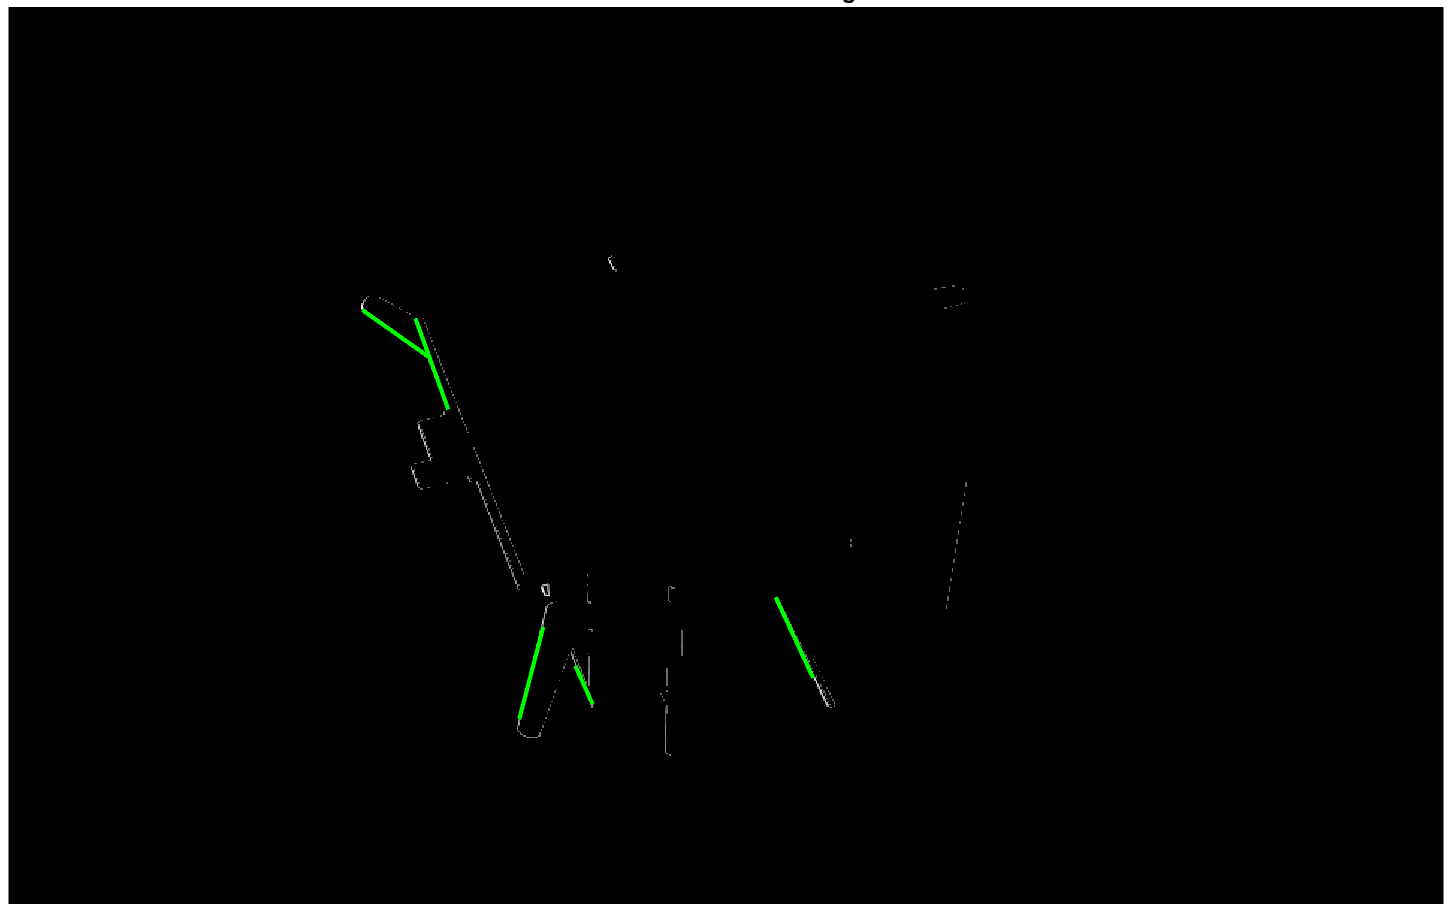
\includegraphics[width=0.47\textwidth]{gfx/FeatureDetection/192/10.png}}
  \qquad
  \subfloat[\acrshort{seh} stream output.]{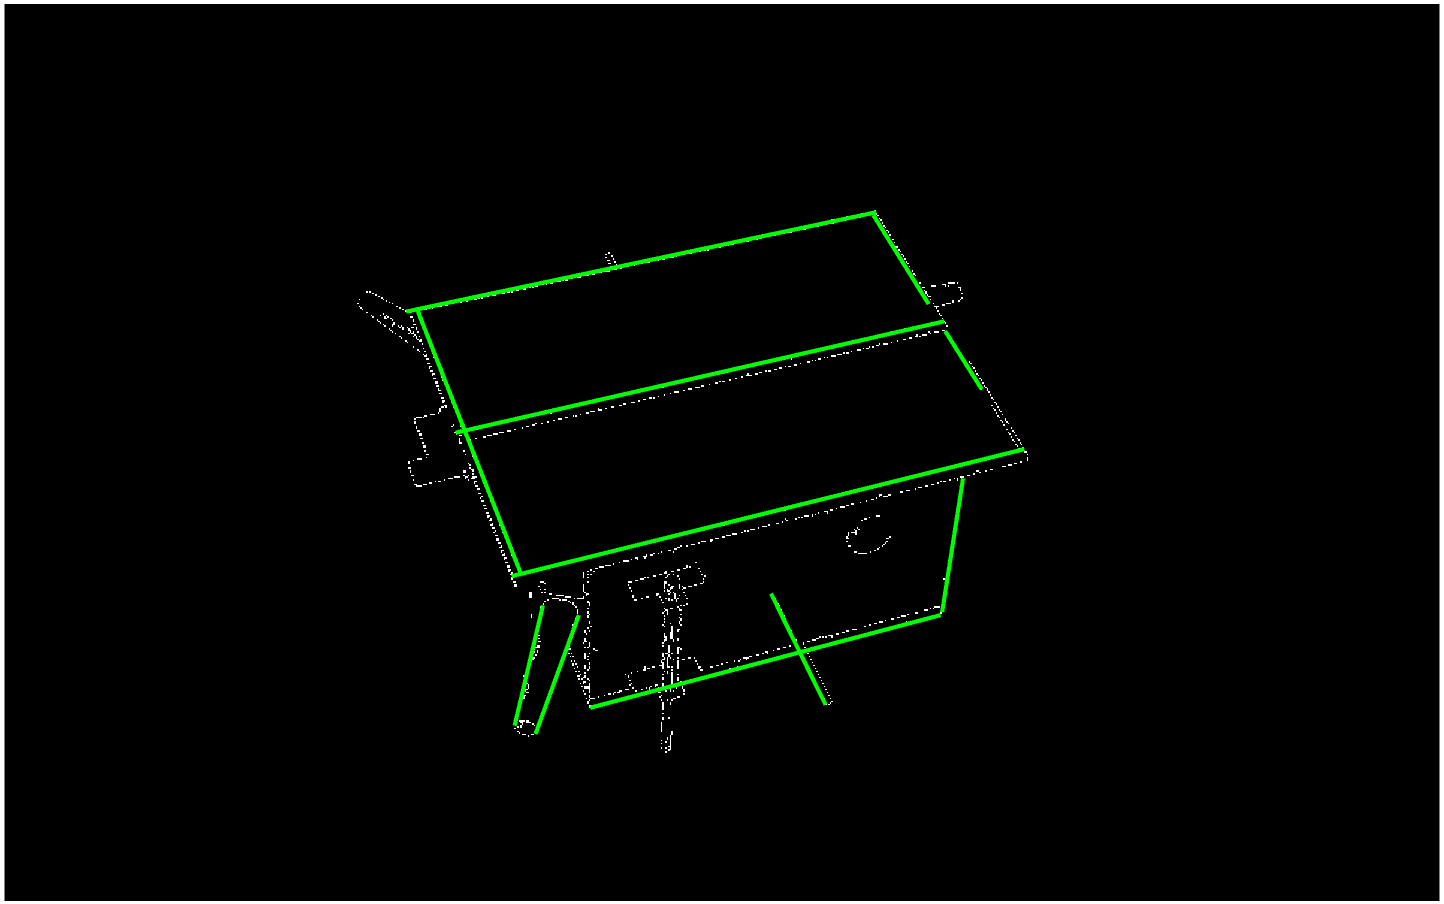
\includegraphics[width=0.47\textwidth]{gfx/FeatureDetection/192/11.png}}
  \qquad
  \subfloat[\acrshort{wge} stream output after merging truncated edges.]{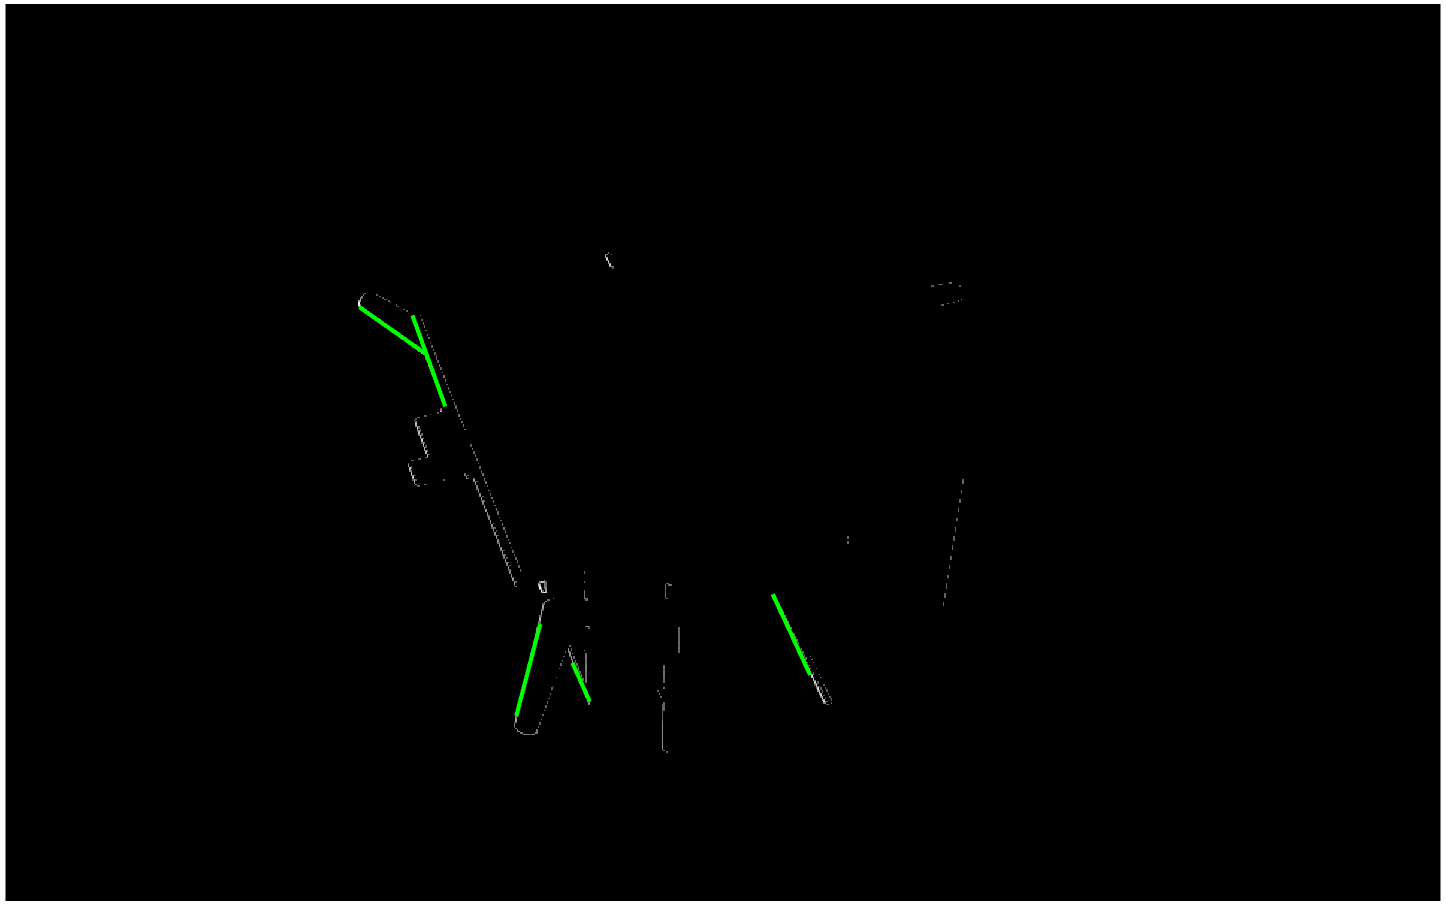
\includegraphics[width=0.47\textwidth]{gfx/FeatureDetection/192/12.png}}
  \qquad
  \subfloat[\acrshort{seh} stream output after merging truncated edges.]{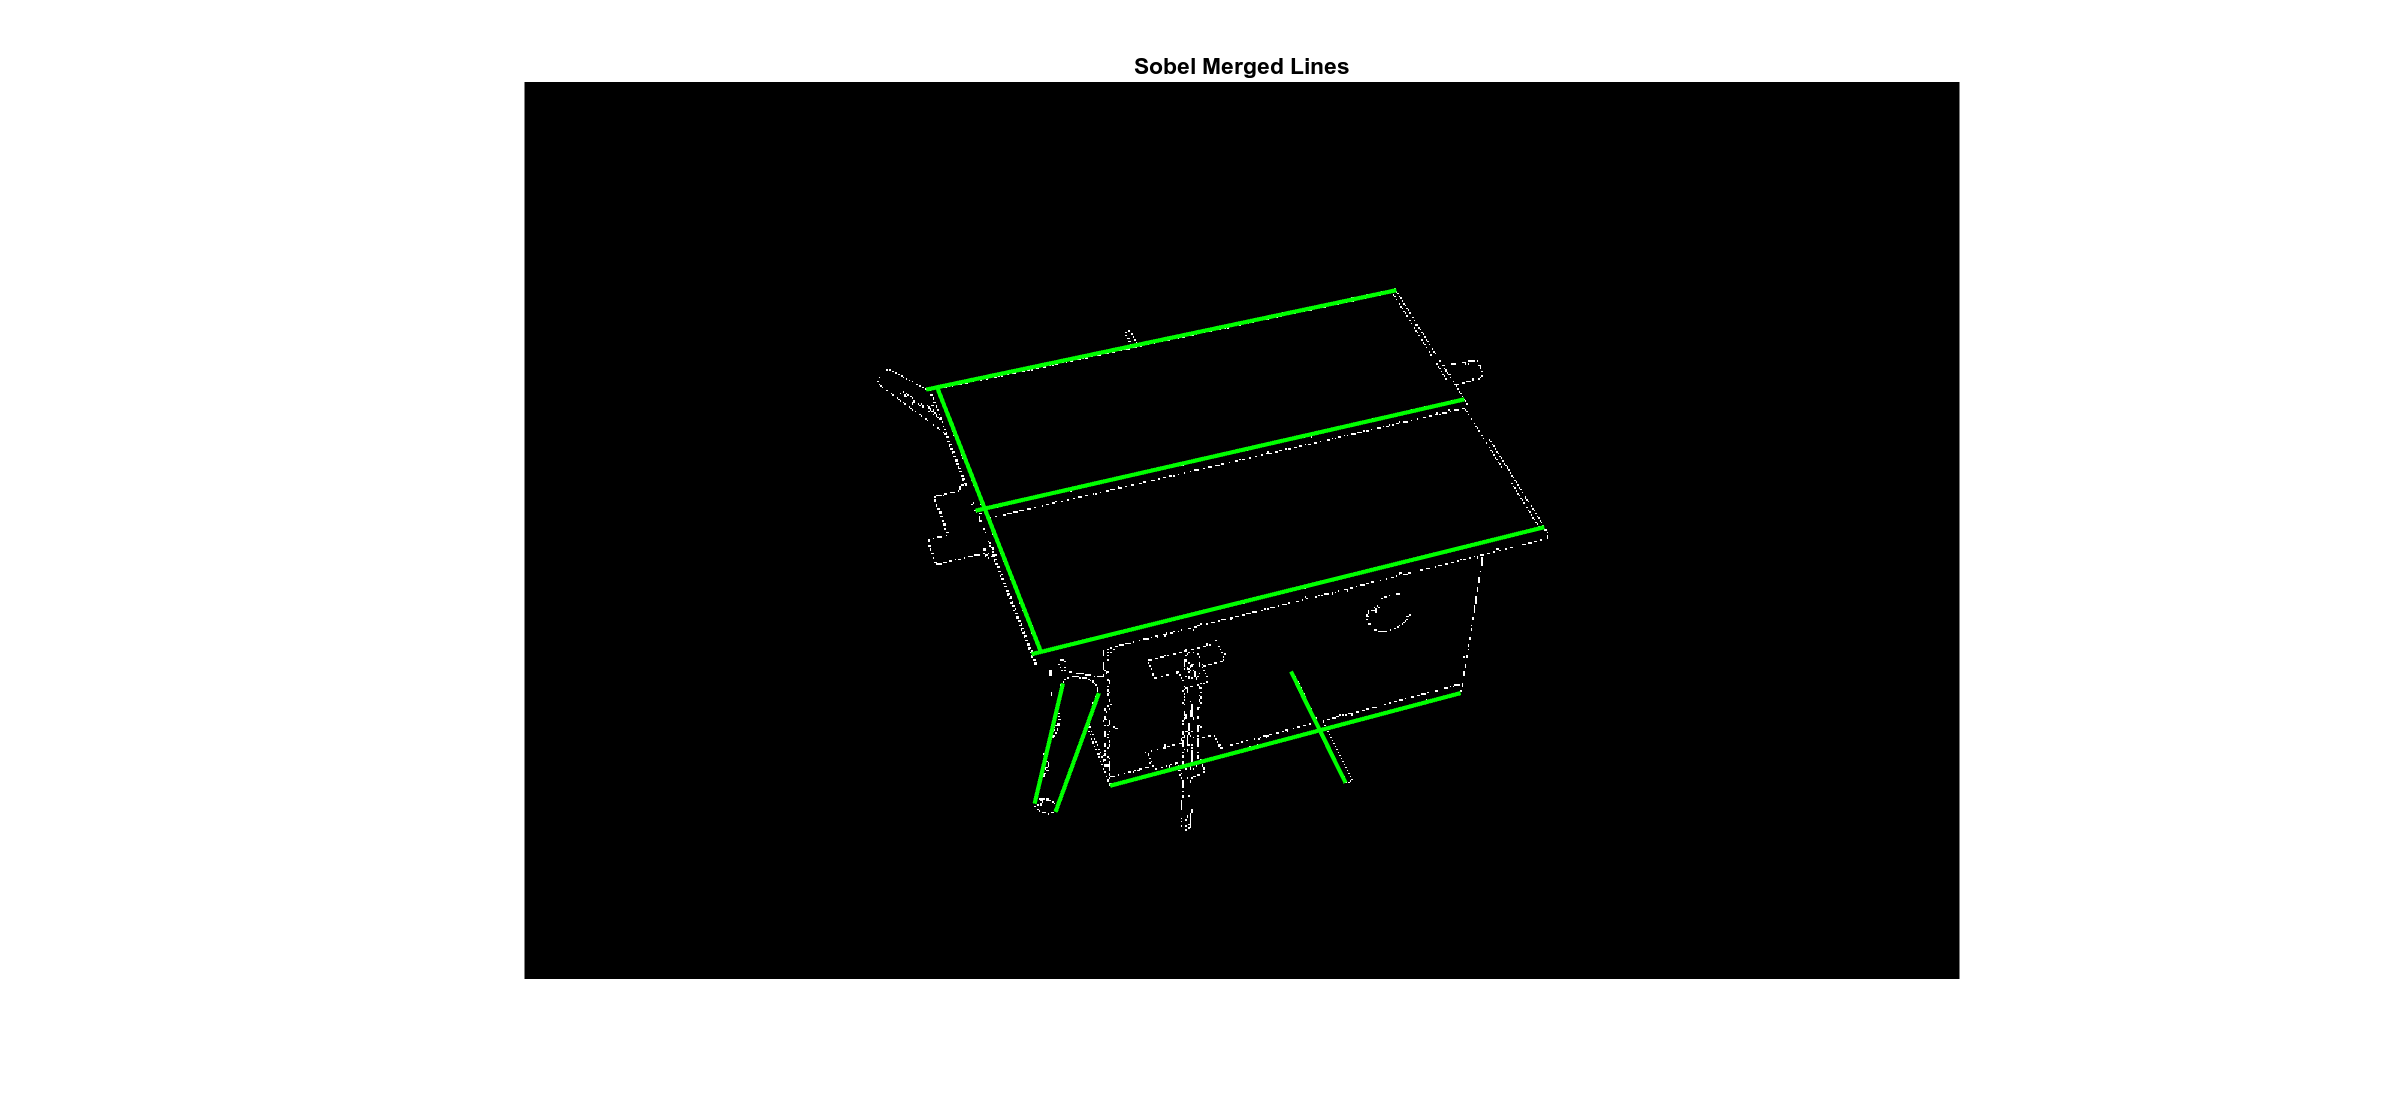
\includegraphics[width=0.47\textwidth]{gfx/FeatureDetection/192/13.png}}
  \qquad
  \subfloat[\acrshort{wge} and \acrshort{seh} streams prior the merge stream procedure.]{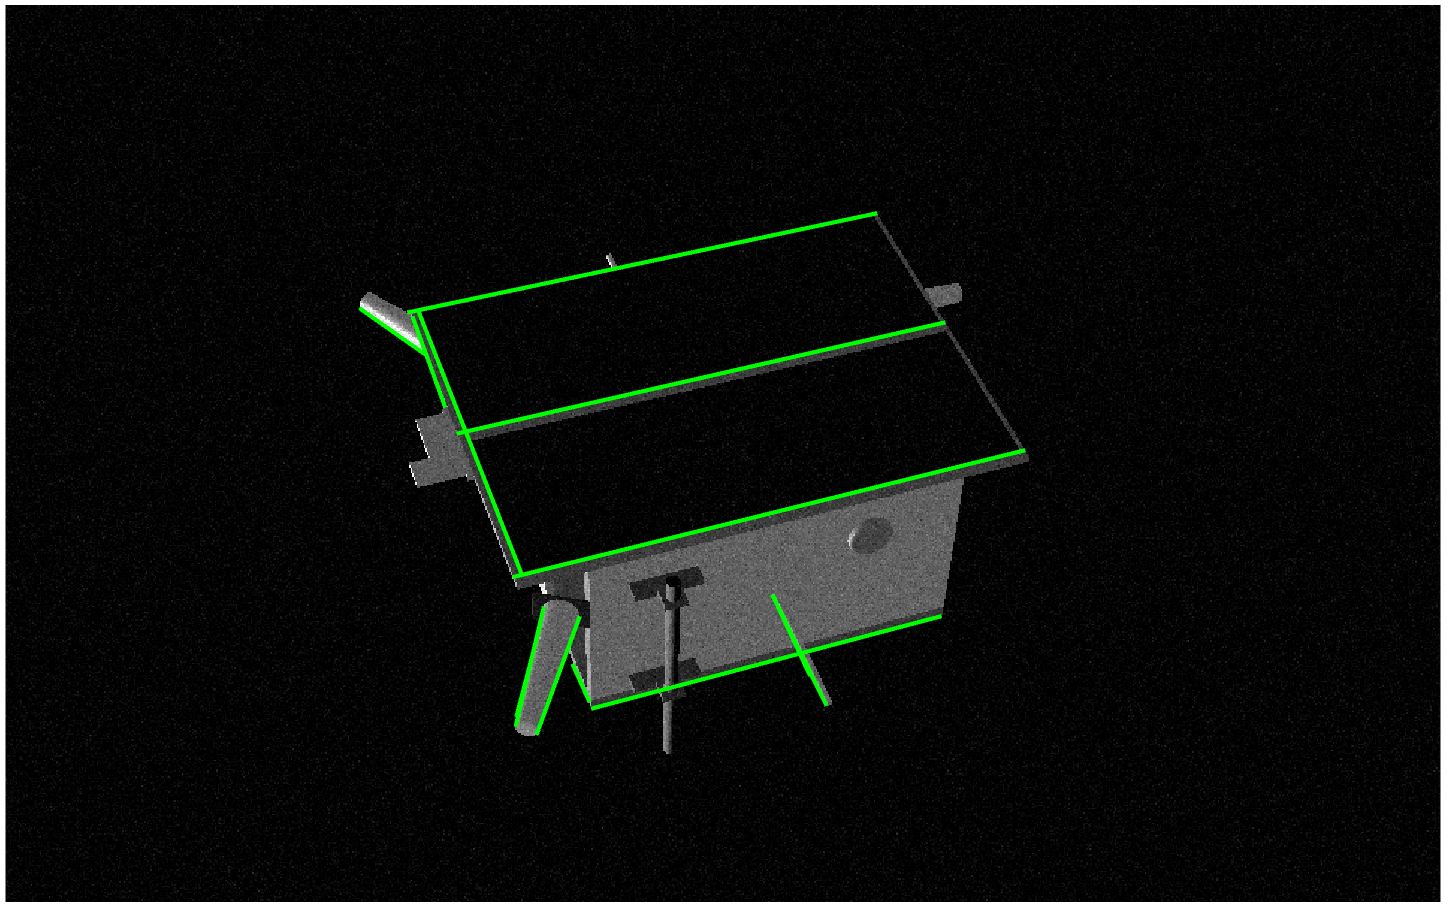
\includegraphics[width=0.47\textwidth]{gfx/FeatureDetection/192/14.png}}
  \qquad
  \subfloat[\acrshort{wge} and \acrshort{seh} streams after the merge stream procedure.]{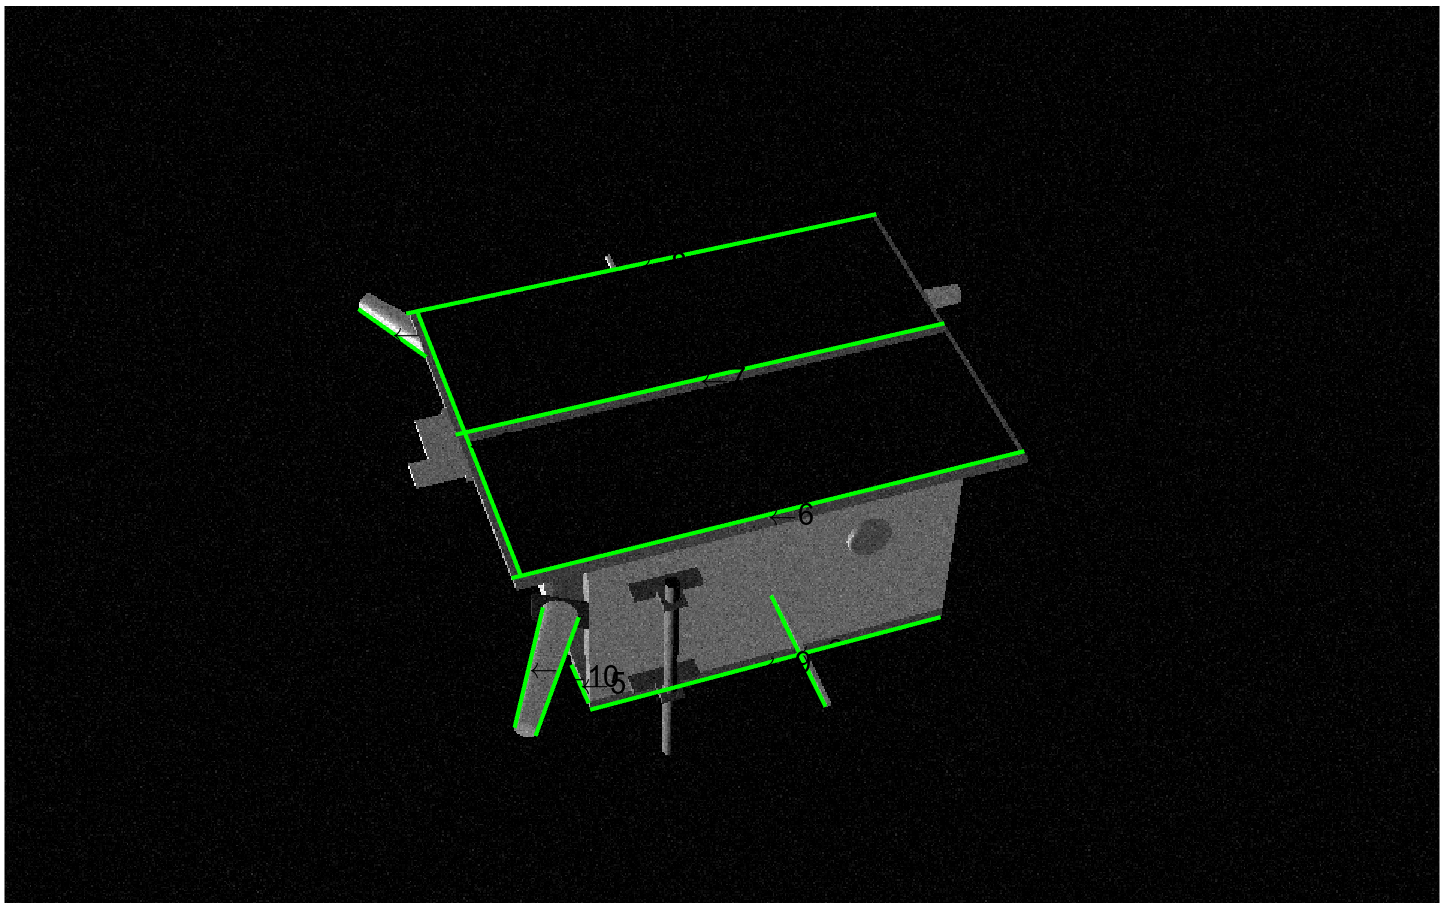
\includegraphics[width=0.47\textwidth]{gfx/FeatureDetection/192/15.png}}
  \qquad
  \caption{Outputs of the image processing subsystem (1).}
  \label{fig:mergeStreams1}
\end{figure}

\begin{figure}[htbp]
  \centering
  \subfloat[\acrshort{wge} stream output.]{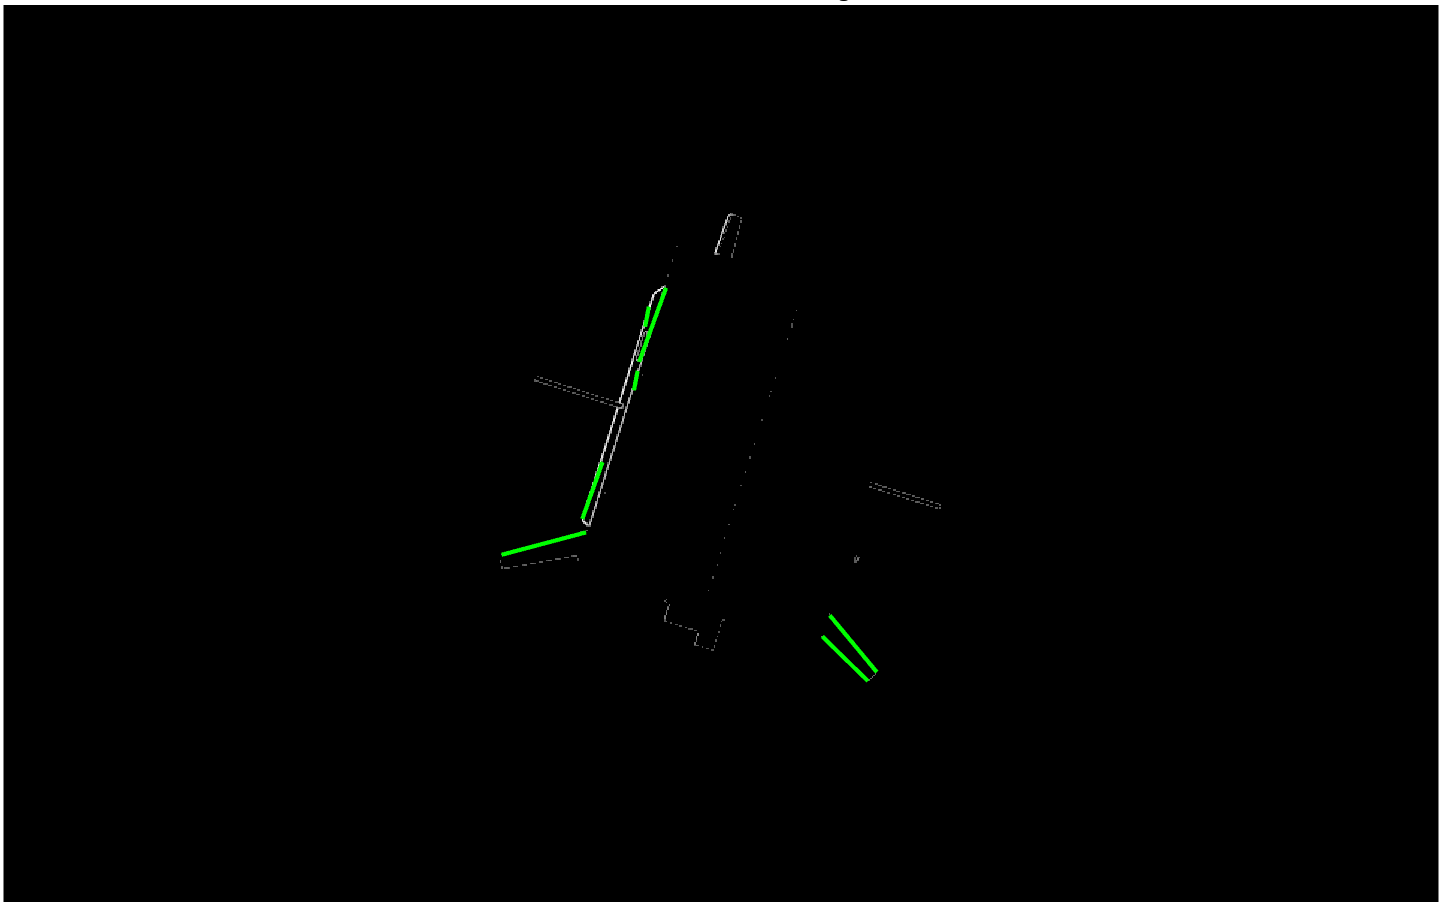
\includegraphics[width=0.47\textwidth]{gfx/FeatureDetection/214/10.png}}
  \qquad
  \subfloat[\acrshort{seh} stream output.]{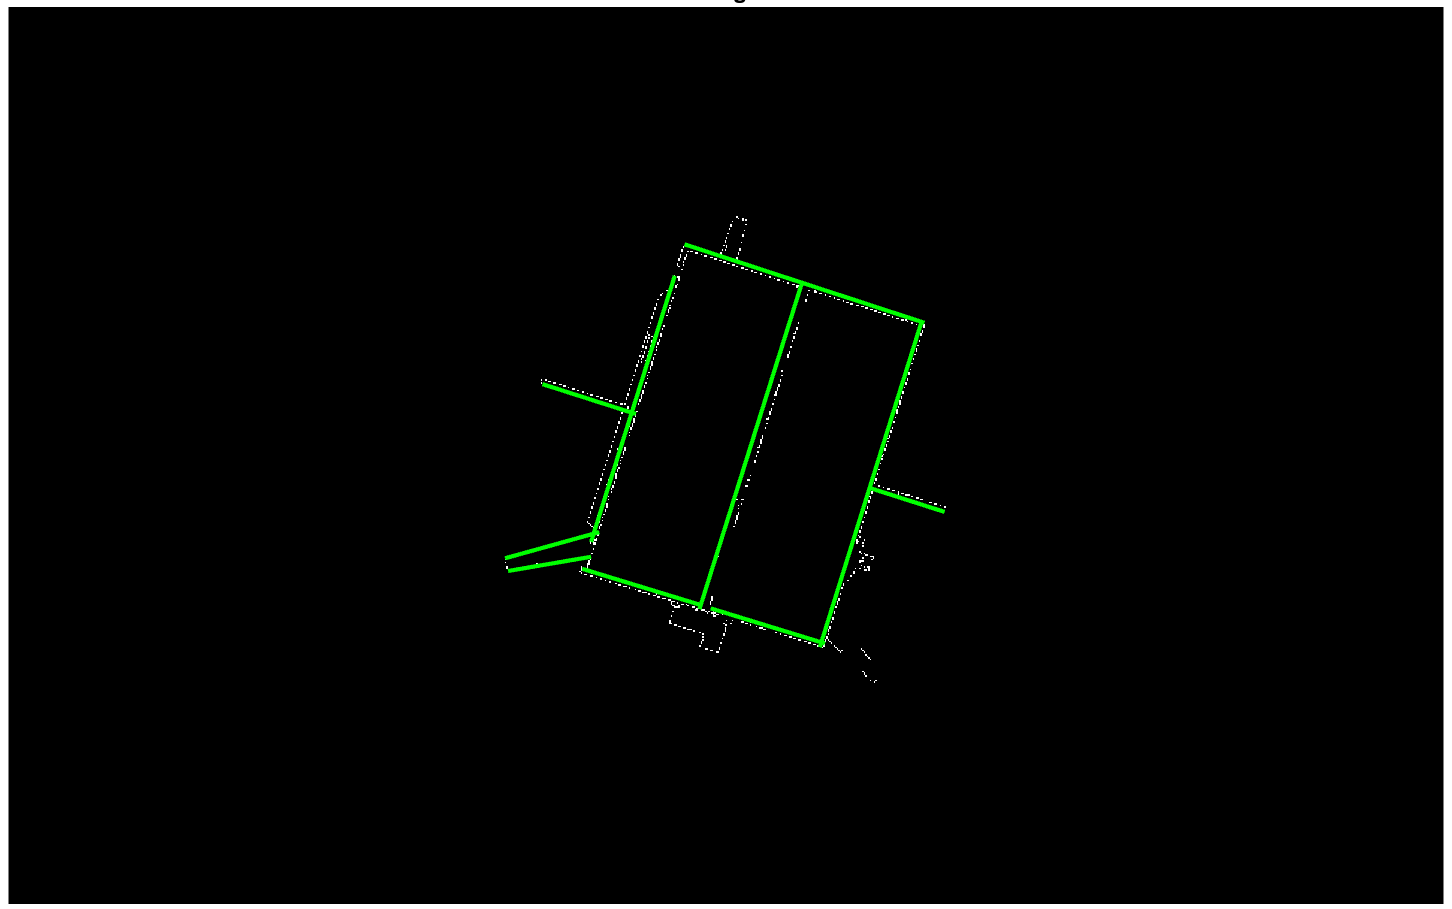
\includegraphics[width=0.47\textwidth]{gfx/FeatureDetection/214/11.png}}
  \qquad
  \subfloat[\acrshort{wge} stream output after merging truncated edges.]{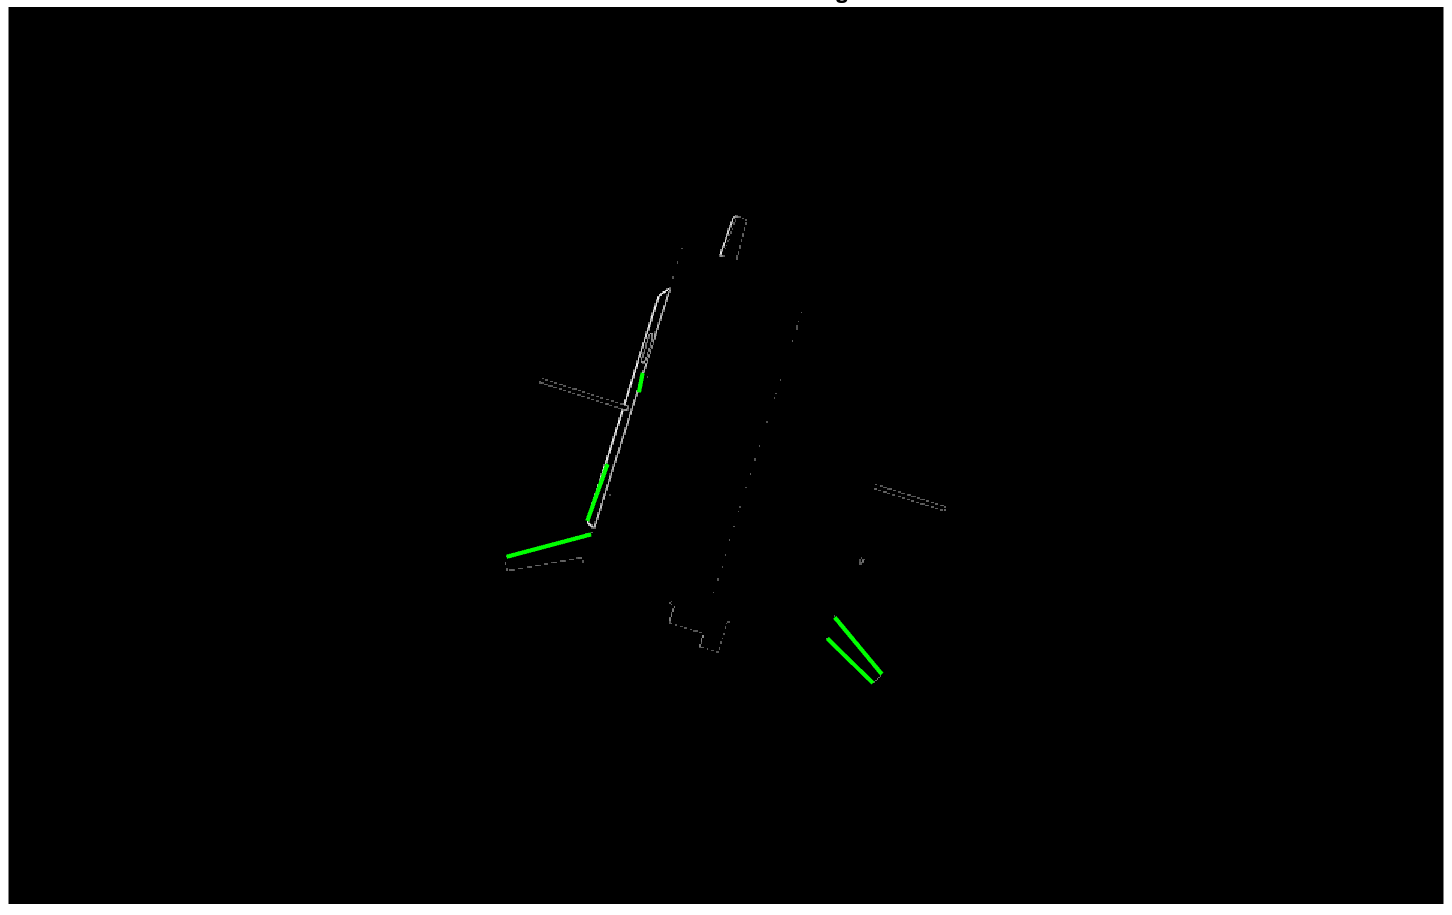
\includegraphics[width=0.47\textwidth]{gfx/FeatureDetection/214/12.png}}
  \qquad
  \subfloat[\acrshort{seh} stream output after merging truncated edges.]{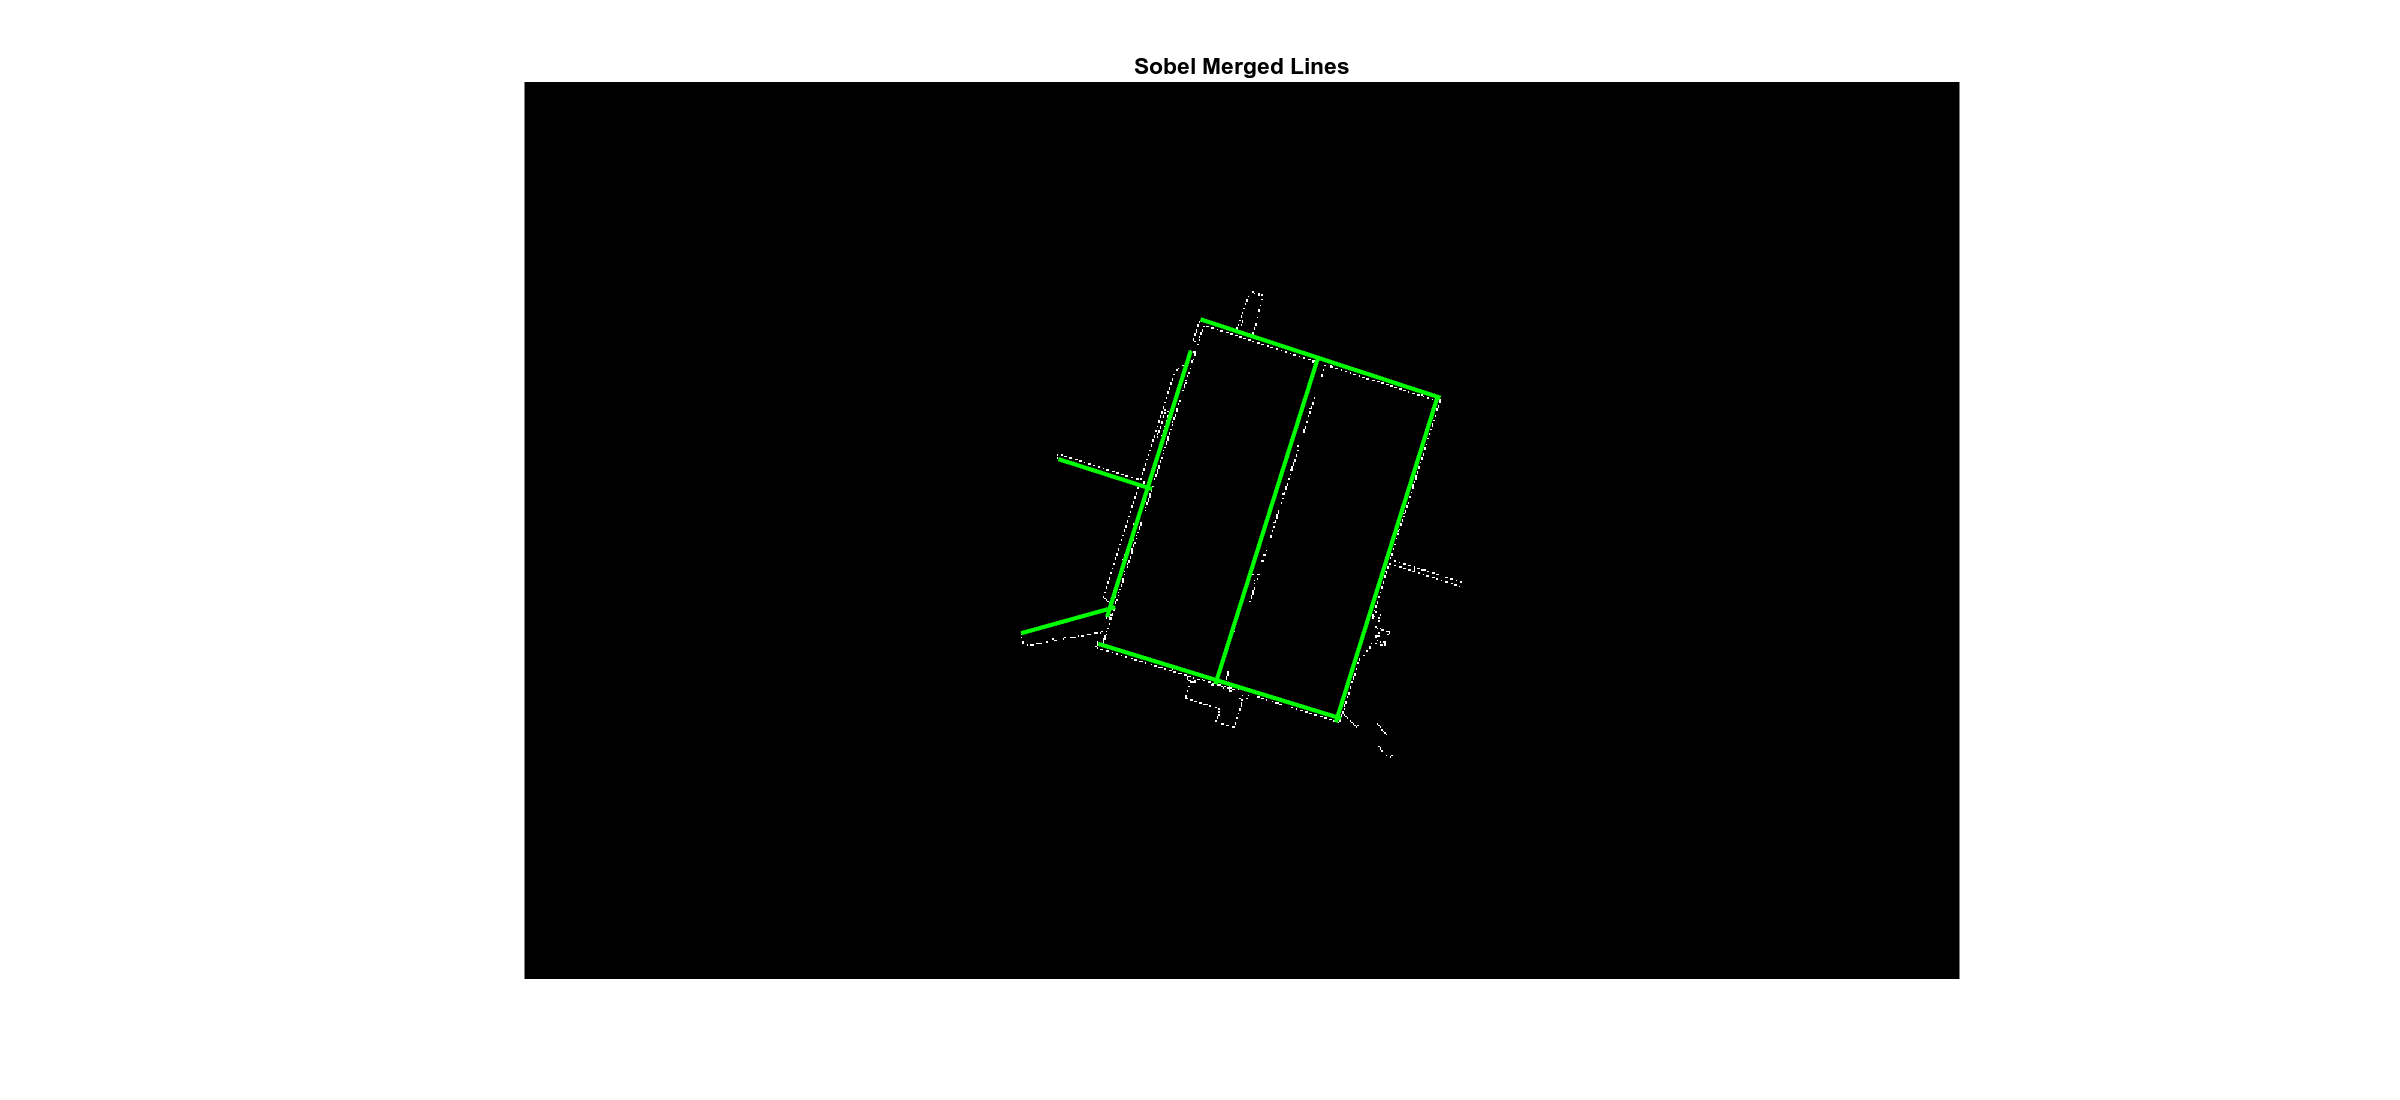
\includegraphics[width=0.47\textwidth]{gfx/FeatureDetection/214/13.png}}
  \qquad
  \subfloat[\acrshort{wge} and \acrshort{seh} streams prior the merge stream procedure.]{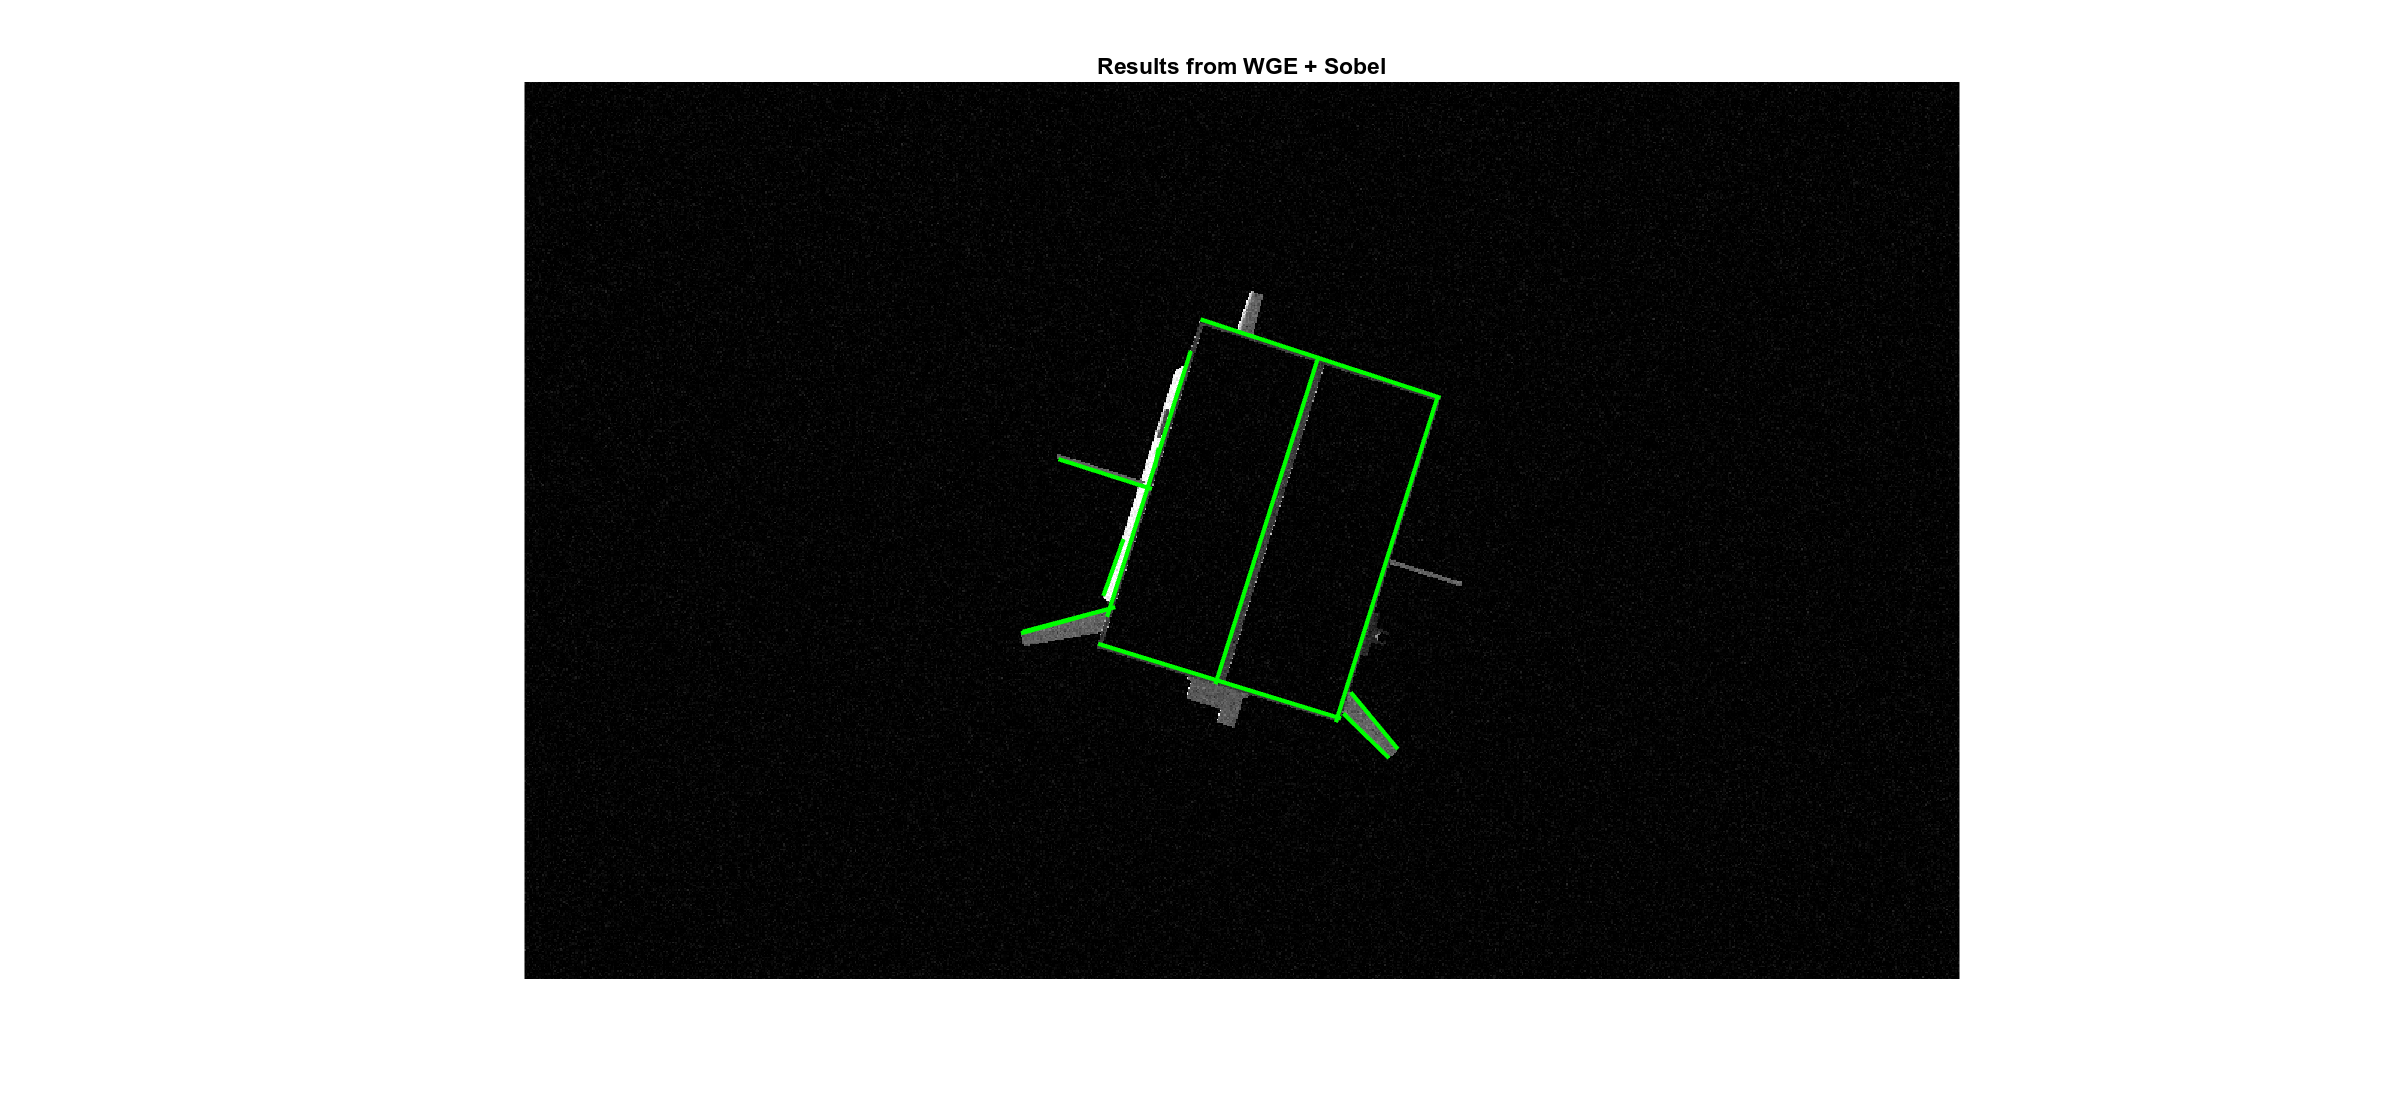
\includegraphics[width=0.47\textwidth]{gfx/FeatureDetection/214/14.png}}
  \qquad
  \subfloat[\acrshort{wge} and \acrshort{seh} streams after the merge stream procedure.]{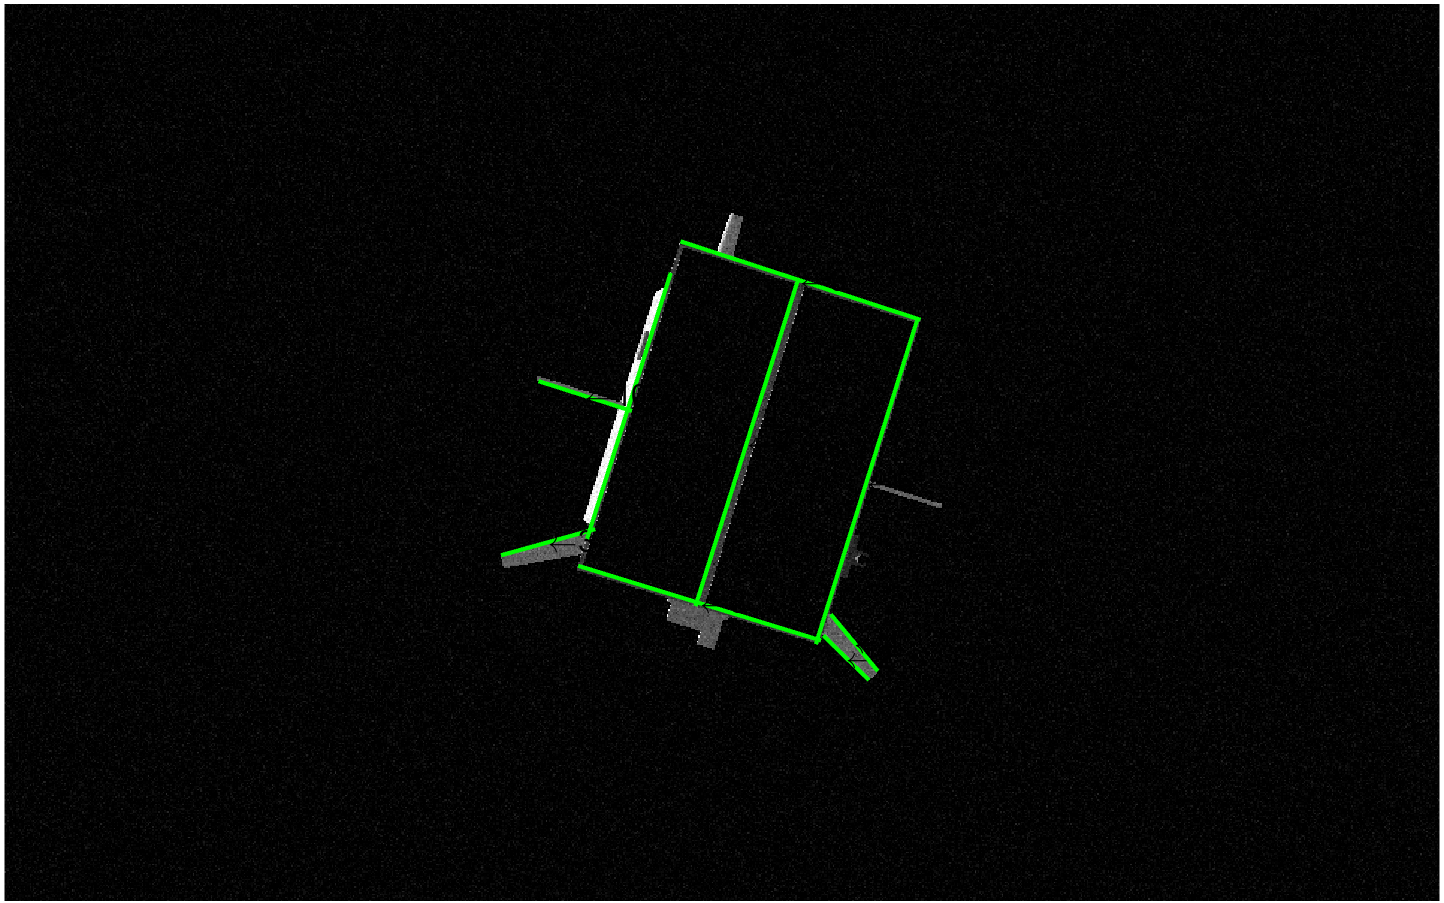
\includegraphics[width=0.47\textwidth]{gfx/FeatureDetection/214/15.png}}
  \qquad
  \caption{Outputs of the image processing subsystem (2).}
  \label{fig:mergeStreams2}
\end{figure}

\begin{figure}[htbp]
  \centering
  \subfloat[\acrshort{wge} stream output.]{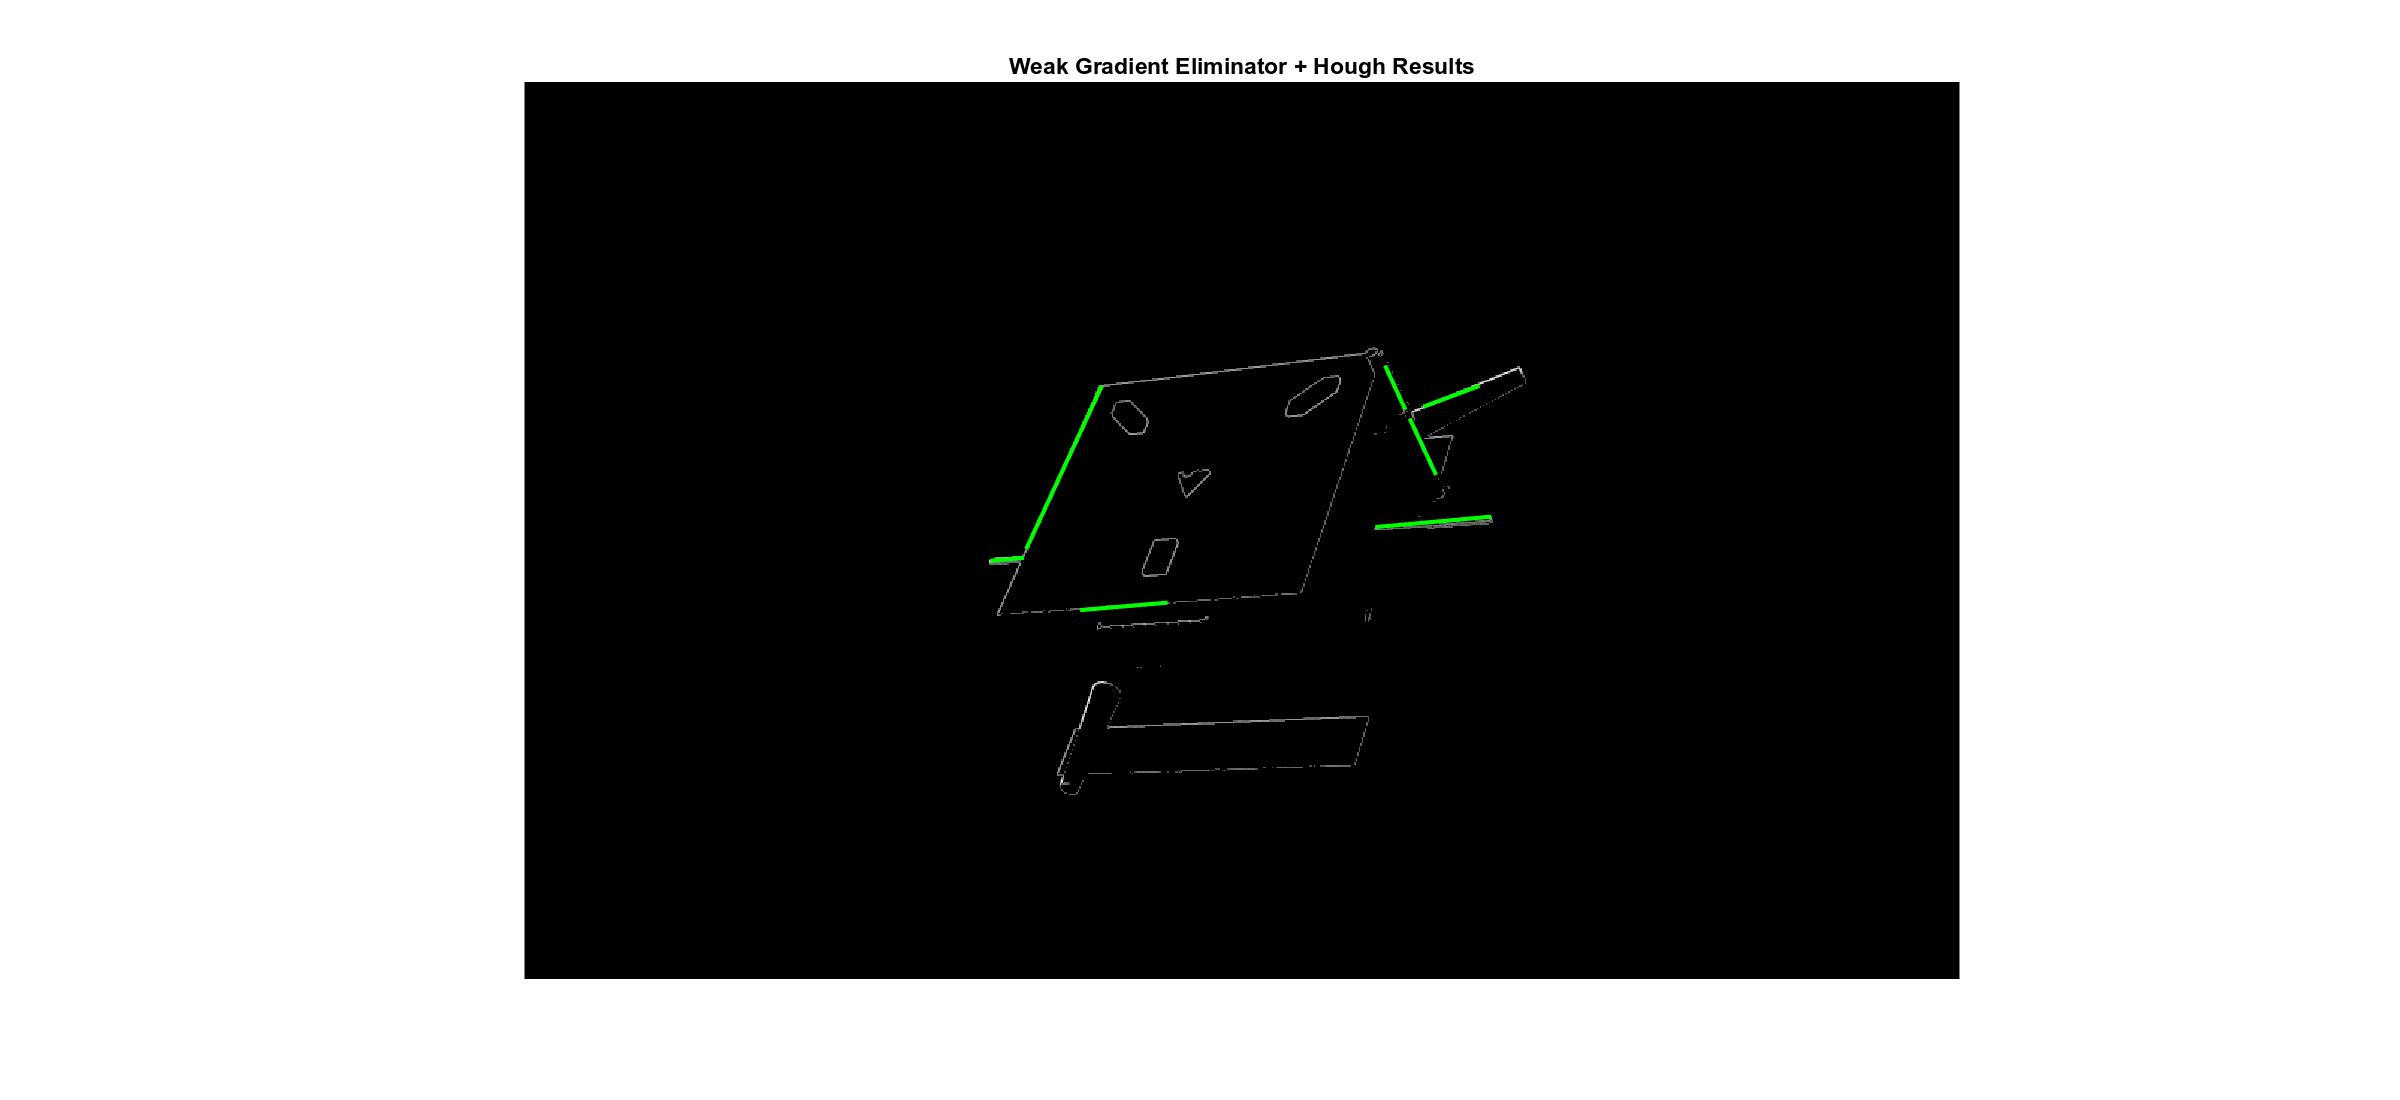
\includegraphics[width=0.47\textwidth]{gfx/FeatureDetection/311/10.png}}
  \qquad
  \subfloat[\acrshort{seh} stream output.]{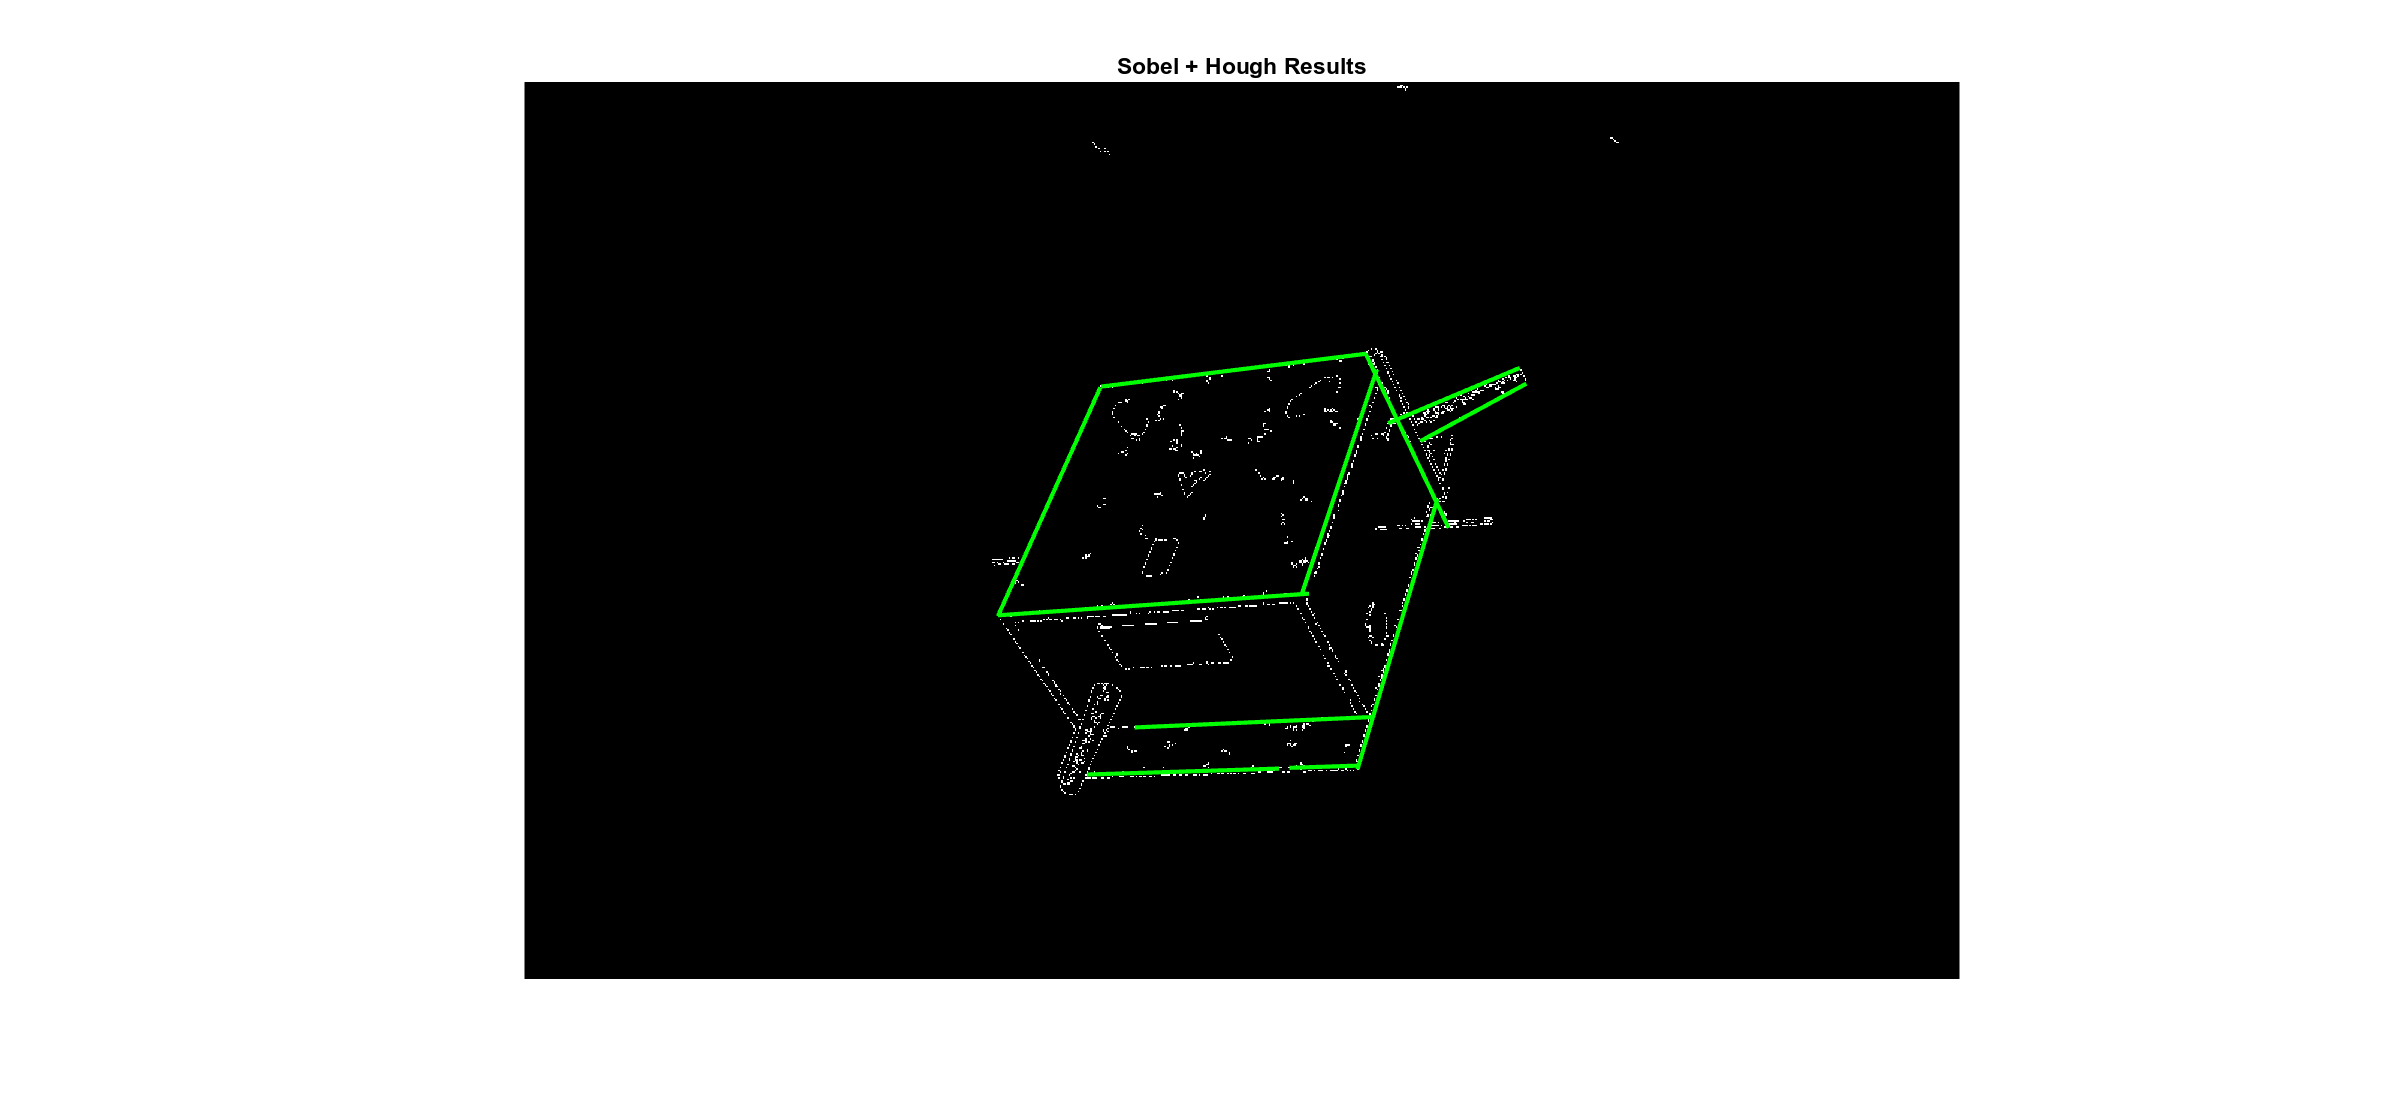
\includegraphics[width=0.47\textwidth]{gfx/FeatureDetection/311/11.png}}
  \qquad
  \subfloat[\acrshort{wge} stream output after merging truncated edges.]{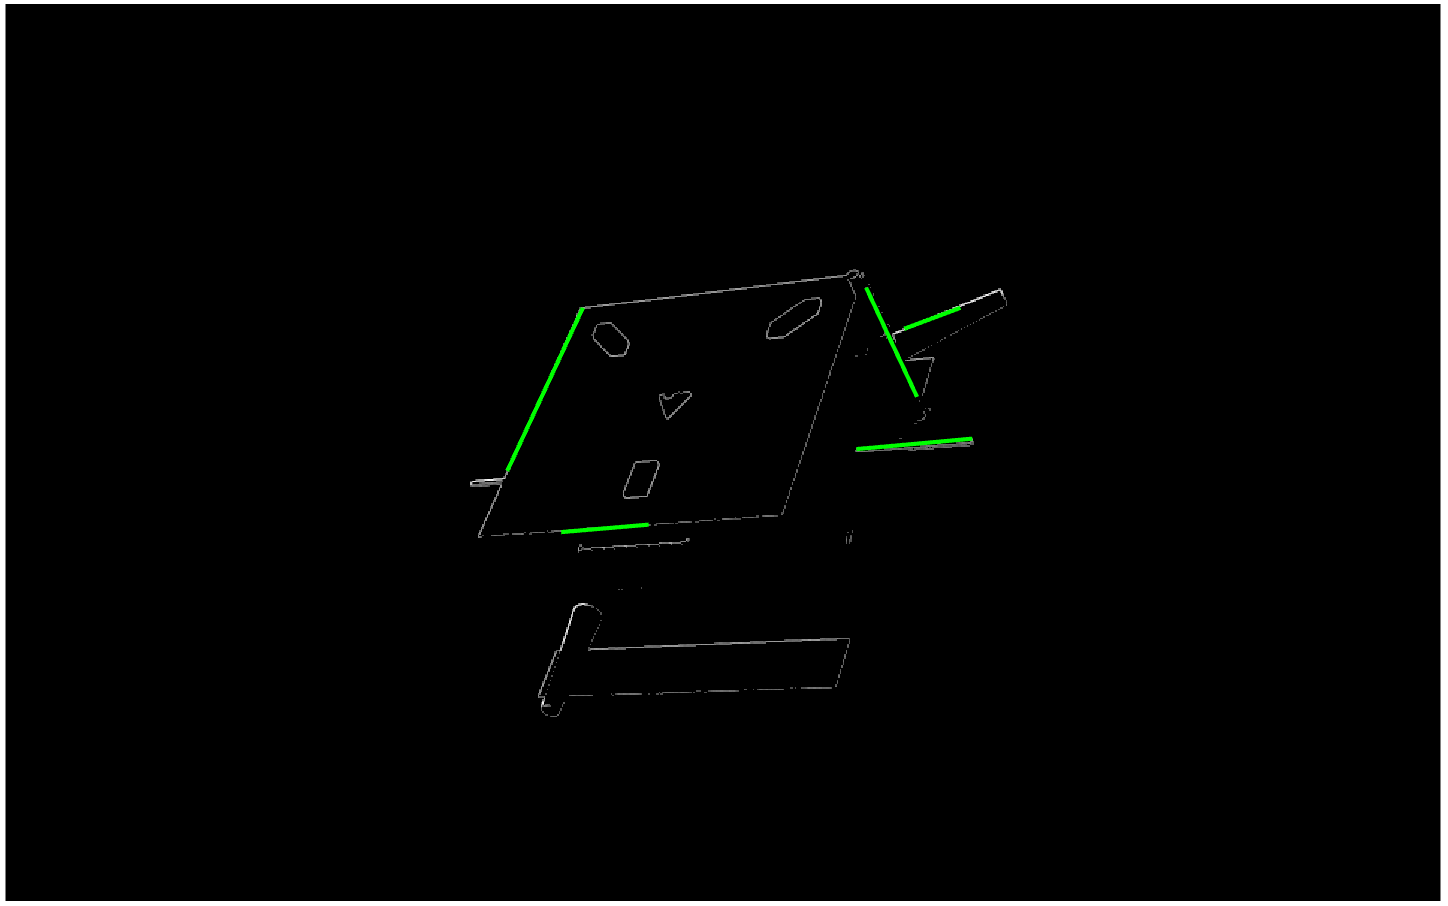
\includegraphics[width=0.47\textwidth]{gfx/FeatureDetection/311/12.png}}
  \qquad
  \subfloat[\acrshort{seh} stream output after merging truncated edges.]{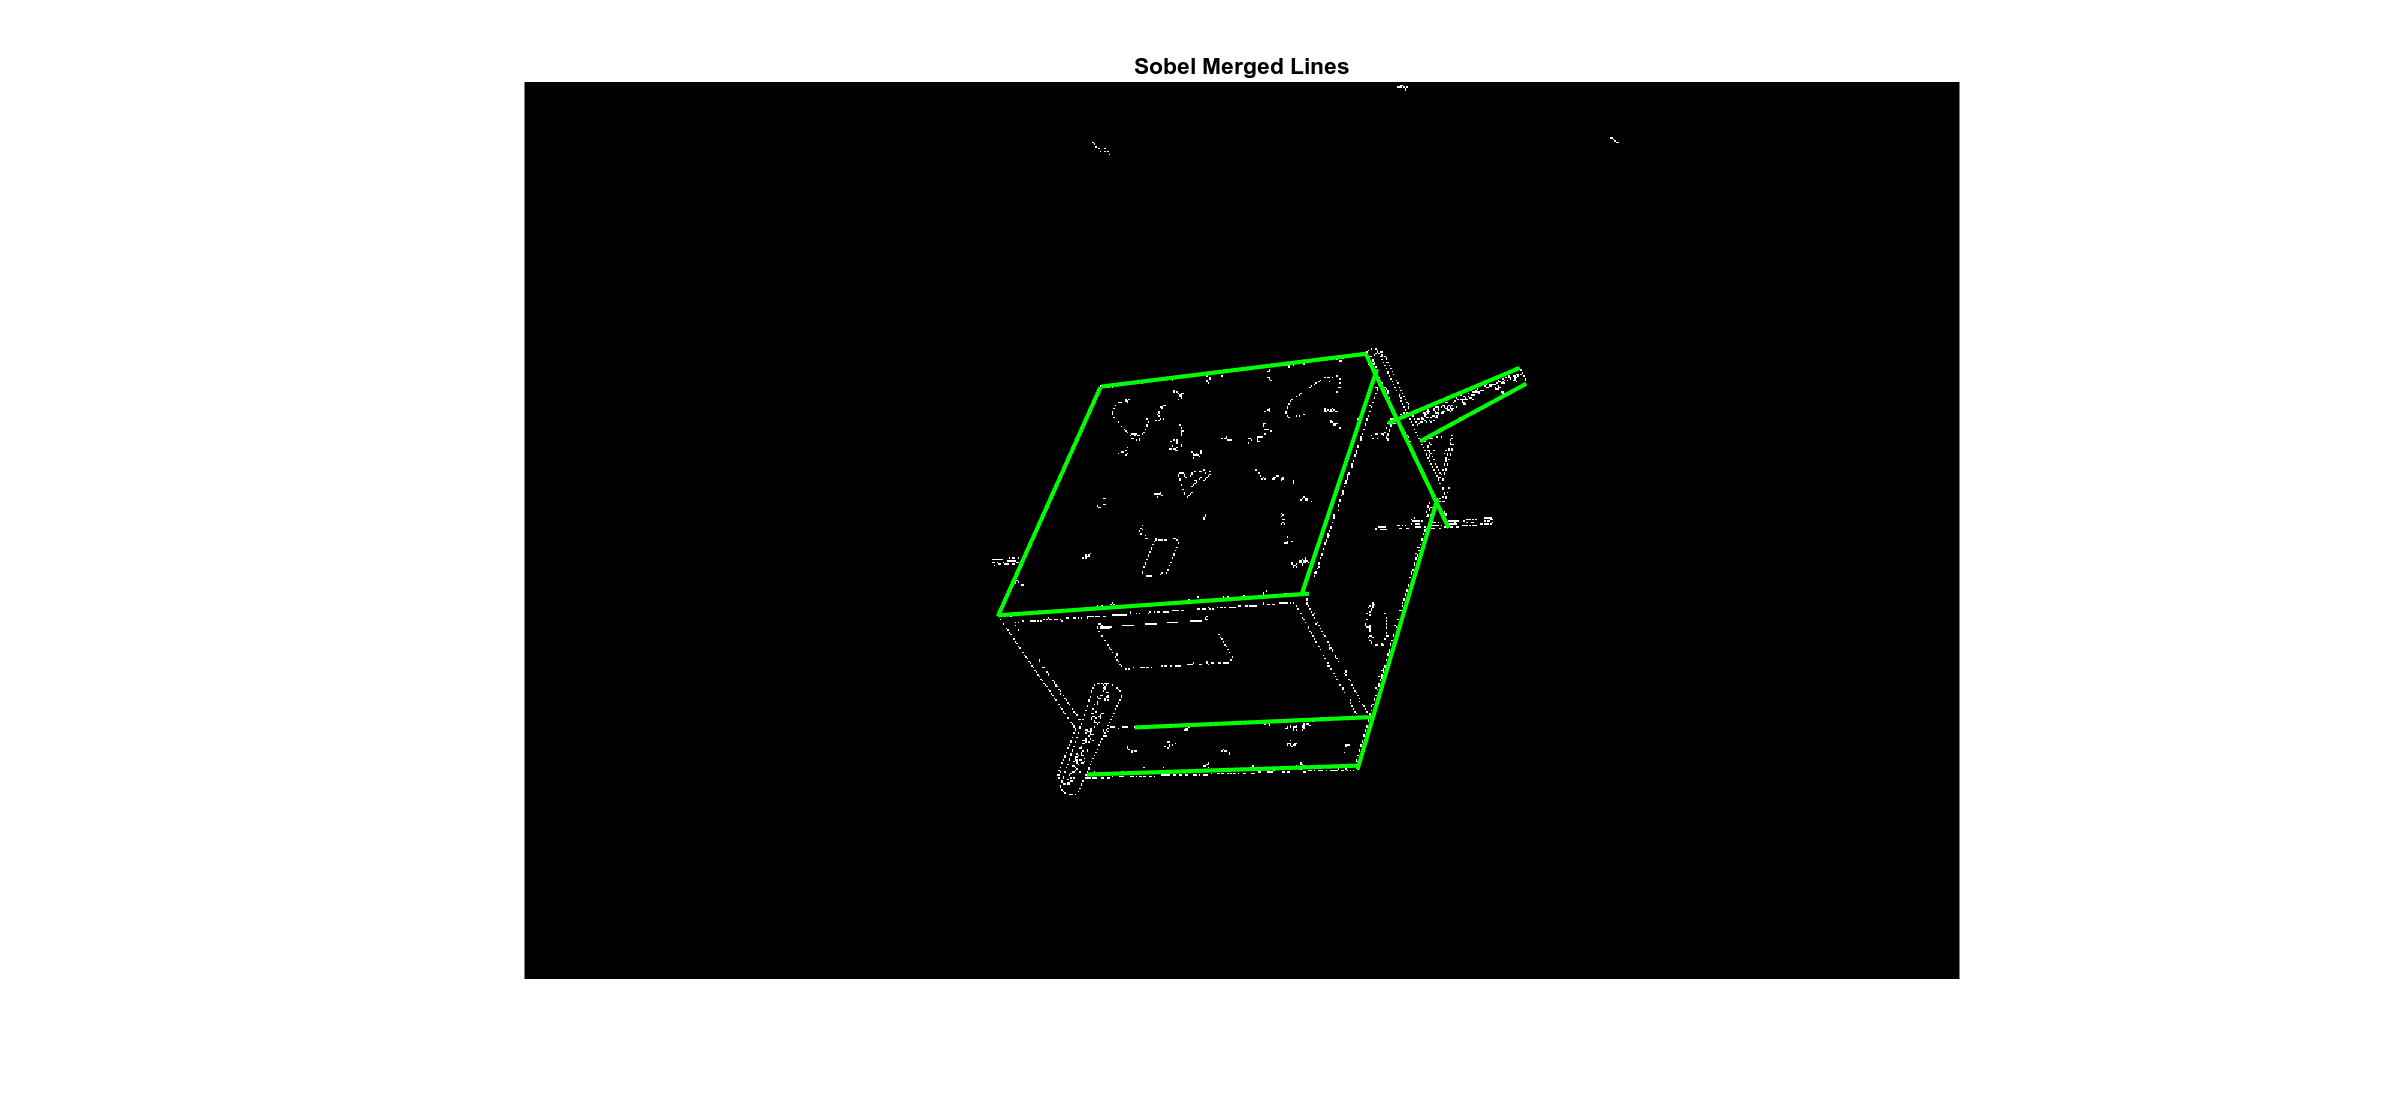
\includegraphics[width=0.47\textwidth]{gfx/FeatureDetection/311/13.png}}
  \qquad
  \subfloat[\acrshort{wge} and \acrshort{seh} streams prior the merge stream procedure.]{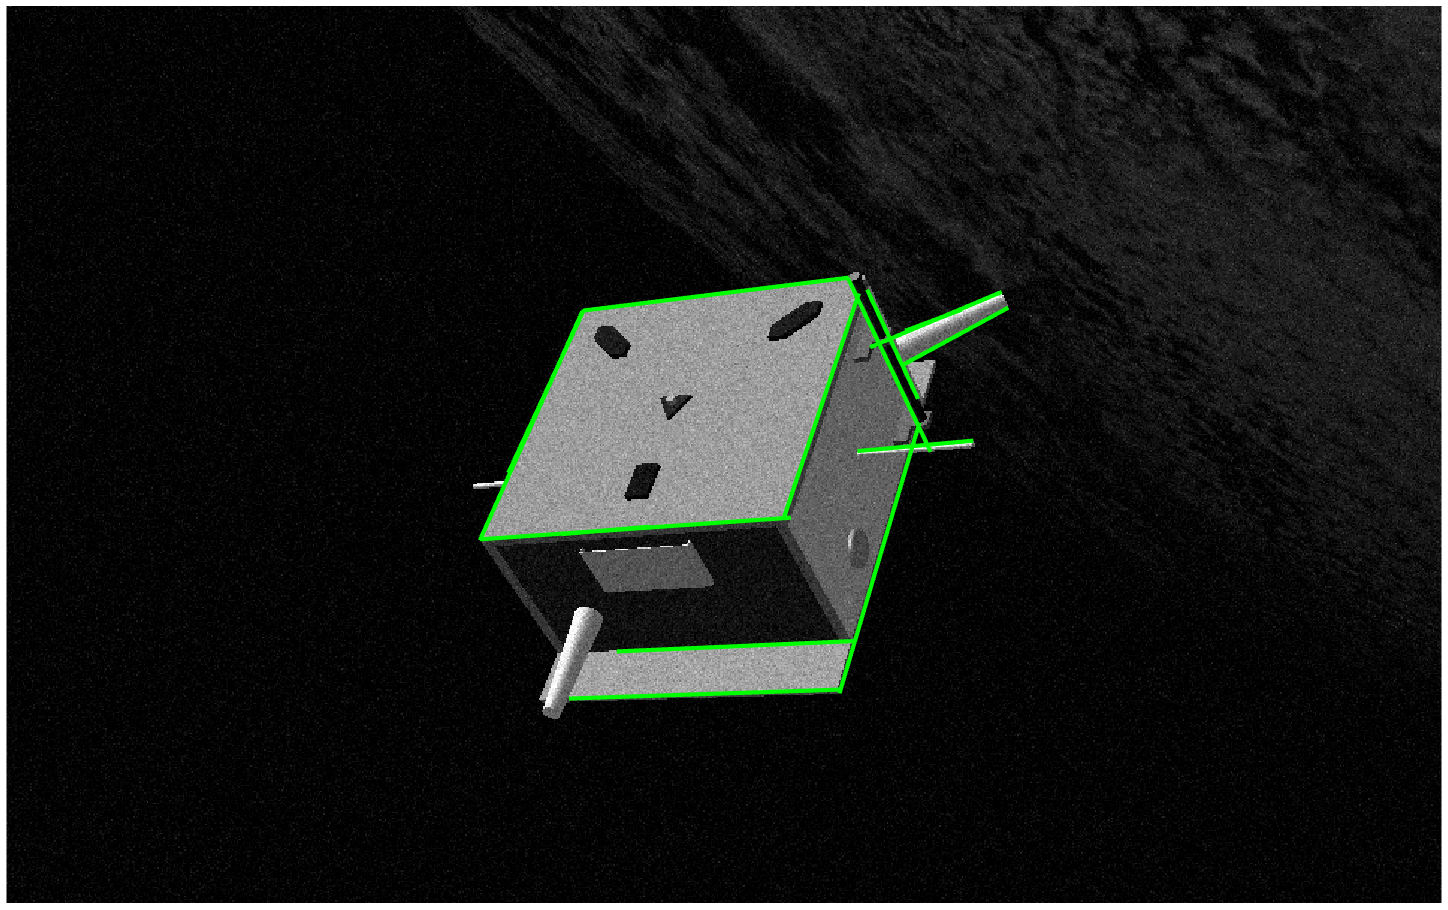
\includegraphics[width=0.47\textwidth]{gfx/FeatureDetection/311/14.png}}
  \qquad
  \subfloat[\acrshort{wge} and \acrshort{seh} streams after the merge stream procedure.]{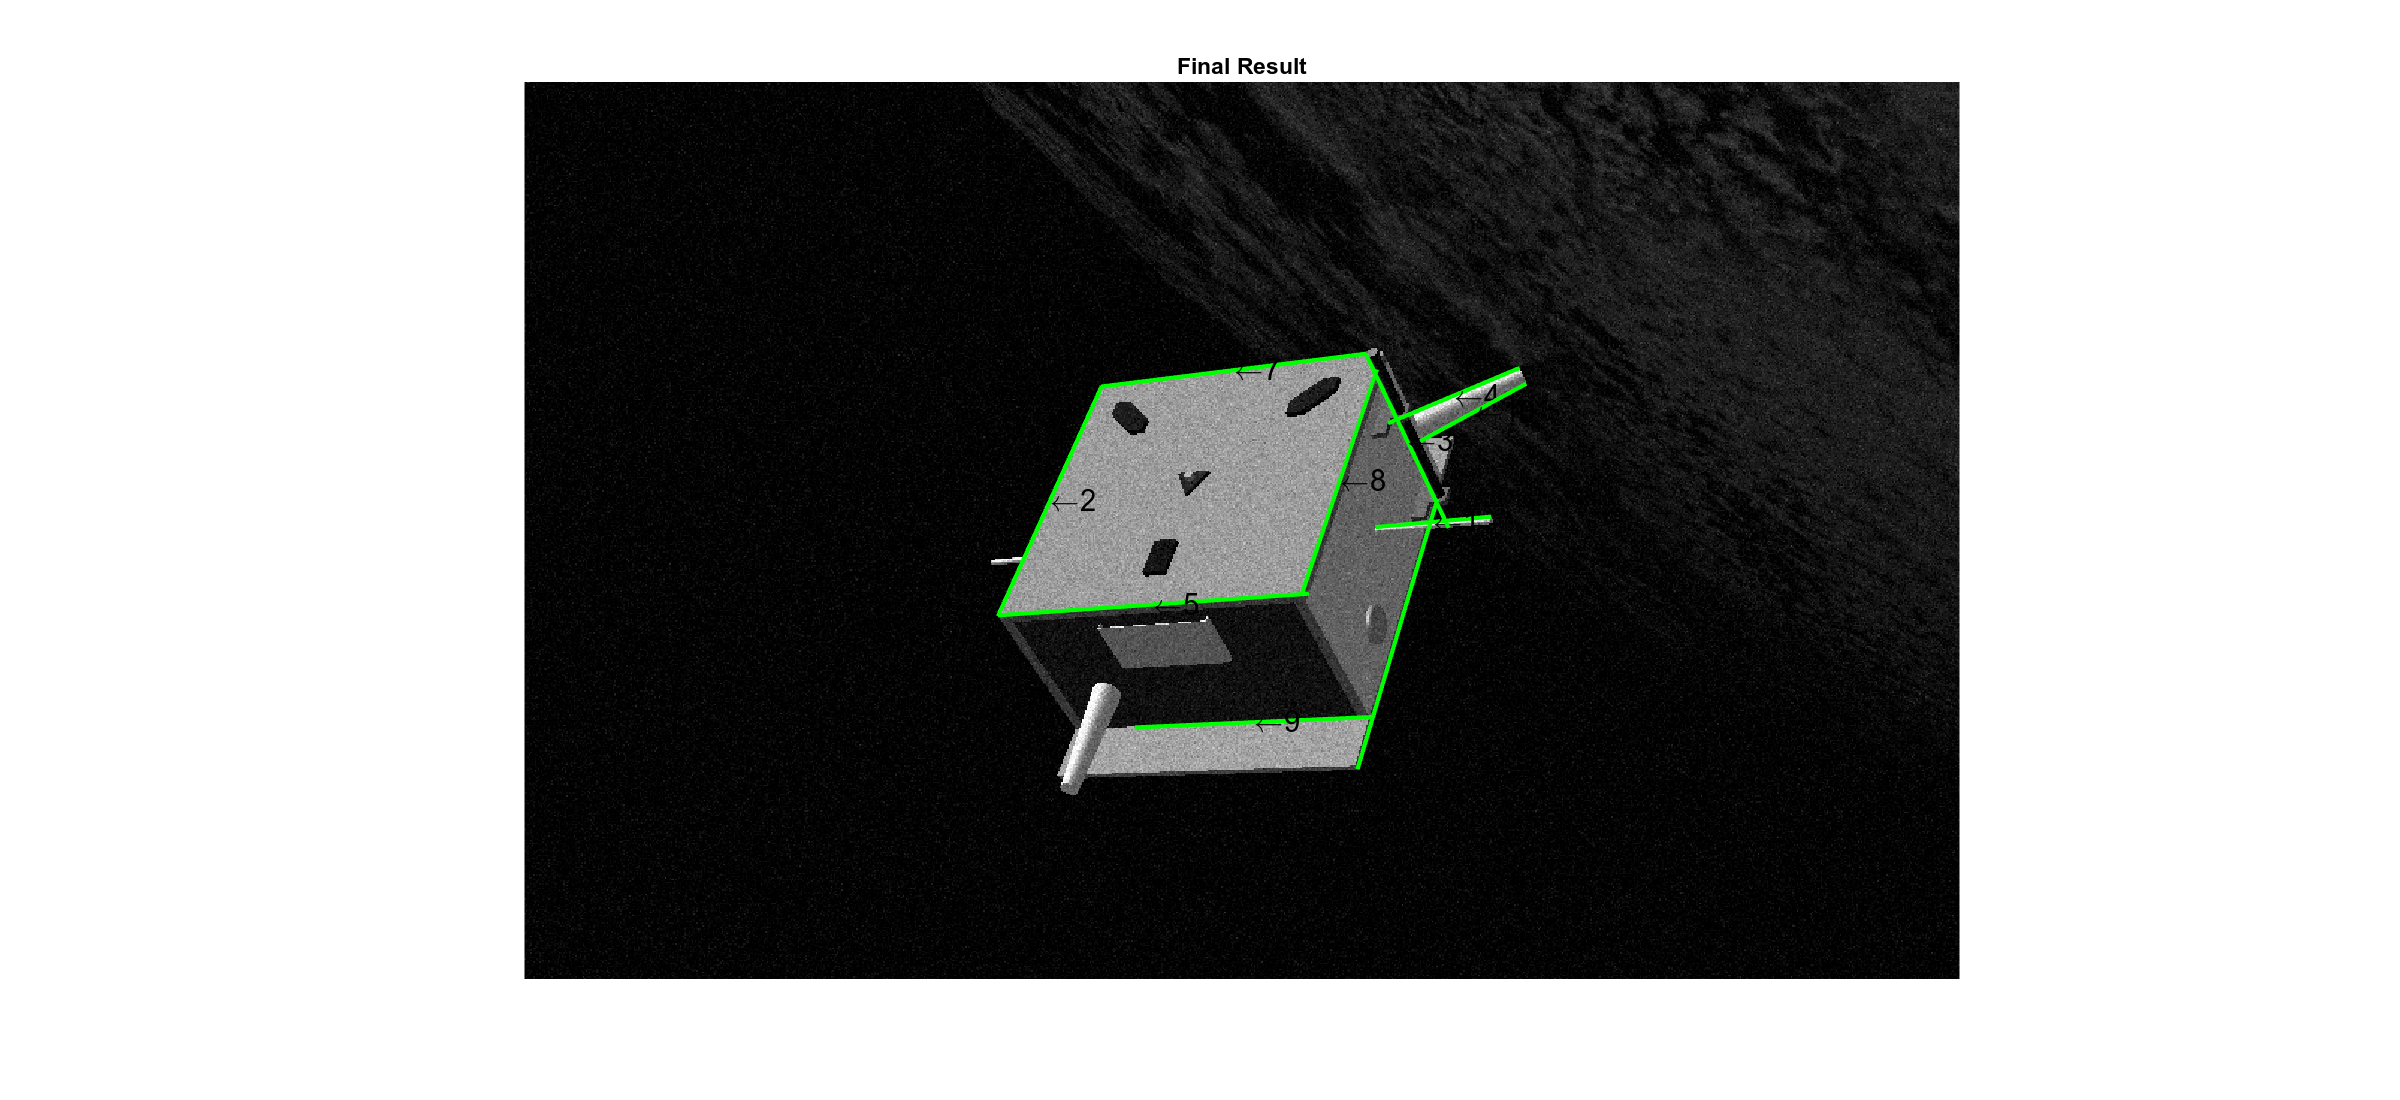
\includegraphics[width=0.47\textwidth]{gfx/FeatureDetection/311/15.png}}
  \qquad
  \caption{Outputs of the image processing subsystem (3).}
  \label{fig:mergeStreams3}
\end{figure}

\subsubsection{Feature Synthesis and Perceptual Grouping}
One of the innovation introduced in the \acrshort{svd} algorithm is what by the original authors has been defined as "Feature Synthesys", which allows to organize the simple segments output from the merge of the \acrshort{wge} and \acrshort{seh} streams into high-level geometrical groups called "Perceptual Groups" in order to reduce the search space of the correspondence problem. Being able to correctly define perceptual groups is of crucial importance to have a successful pose initialization.
As stated in \cite{10.1145/358669.358692}, to uniquely solve the \acrshort{pnp} problem are required at least six correspondences between model and image points. The number of possible correspondences, so, the number of hypothetical pose solution given \textit{n} points in the image and \textit{m} points in the \acrshort{3d} model therefore can be expressed as \cite{Sharma2018}:

\begin{equation*}
  \binom{m}{6} \binom{n}{6} 6! \,.
\end{equation*}

The idea presented by Sharma \textit{et al.} so is to reduce the solutions' search space by just using a small set of high level feature groups instead of using a large number of feature point. For example, it is sufficiently safe to say that four image points may belong to a polygonal feature such as a solar panel, then a unique solution can be found by just using four correspondences. The feature synthesis implementation proposed by Sharma \textit{et al.} groups the features into five high-level perceptual groups, which, in order of increasing complexity are:

\begin{itemize}
  \item parallel pairs;
  \item proximity pairs;
  \item parallel triads;
  \item proximity triads;
  \item closed polygonal tetrads;
\end{itemize}

moreover, antennas are treated as a separate feature group.
As done for the merging procedure, the perceptual groups are recognized by examining several geometrical constraints.

\begin{figure}[htbp]
  \centering
  \subfloat[Parallel Pair.]{\includegraphics[width=0.24\textwidth]{gfx/parallelPair.eps}}
  \qquad
  \subfloat[Proximity Pair.]{\includegraphics[width=0.24\textwidth]{gfx/proximityPair.eps}}
  \qquad
  \subfloat[Parallel Triad.]{\includegraphics[width=0.24\textwidth]{gfx/parallelTriad.eps}}
  \qquad
  \subfloat[Proximity Triad.]{\includegraphics[width=0.24\textwidth]{gfx/proximityTriad.eps}}
  \qquad
  \subfloat[Closed Polygonal Tetrad.]{\includegraphics[width=0.24\textwidth]{gfx/closedPolygonalTetrad.eps}}
  \qquad
  \caption{High-level feature groups \cite{Sharma2018}.}
  \label{fig:highLevelGroups}
\end{figure}

Antennas are detected by selecting among all line segments only the one for which the following condition is met:

\begin{equation}
  l_1  \leqslant \tau d_{ROI} \,,
\end{equation}

where $\tau$ is a multiplicative constant, which \cite{Sharma2018} suggests to take equal to $\nicefrac{1}{3}$. Before checking if a line can be inserted into an high level feature group, is always checked if it cannot be characterized as antenna.
With reference to Figure~\ref{fig:highLevelGroups}a, parallelism is enforced by checking the the angular difference between the two line segments:

\begin{equation}
  \theta_{12} = |\theta_1 - \theta_2| \leqslant \theta_{max} \,,
\end{equation}

However, as suggested in \cite{fracchio2019}, to avoid detecting spurious parallel pairs it is useful to introduce two more geometric constraints, which are the minimum radial distance and the minimum lines' length ratio:

\begin{equation}
  \rho_{12} = |\rho_1 - \rho_2| \geq  \rho_{min} \,,
\end{equation}

\begin{equation}
  \epsilon_{12} = \frac{min(l_1,l_2)}{max(l_1,l_2)} \geq \epsilon_{min} \,.
\end{equation}

Proximity pairs instead are detected by checking the distance between their closest endpoints. With reference to Figure ~\ref{fig:highLevelGroups}b, the geometric condition checked is:

\begin{equation}
  d_{12} \leqslant d_{max} \,,
\end{equation}

where $d_{max}$ can be adaptively computed in function of the \acrshort{roi} diagonal length trough a multiplicative constant:

\begin{equation}
  d_{max} = \xi d_{ROI} \,.
\end{equation}

Furthermore, in order to prevent duplicated edges to be grouped as proximal pair, in \cite{fracchio2019} is proposed a supplementary constraint on the minimum angular difference between the two line segments being considered:

\begin{equation}
  \theta_{12} = |\theta_1 - \theta_2| \geq \theta_{min} \,.
\end{equation}

Parallel triads can be detected by selecting among all parallel pairs, the ones which shares a line segment. Similarly, proximity triads are detected by scanning all the proximity pairs and extracting the ones which shares a line segment and satisfy the following geometric condition:

\begin{equation}
  (P_{1a} - P_{3a})(P_{1b}-P_{3b}) > 0 \,.
\end{equation}

Finally, polygonal tetrads that have two segments in common are classified as closed polygonal tetrads.
Similarly, the perceptual grouping is applied to a reduced CAD model of the target \acrshort{sc}. As proposed in \cite{Sharma2018}, the CAD model introduced in Chapter~\ref{chap:second-chapter} is reduced to only contain a low number of features. The number of features present in the wireframe reduced modules must be tuned in order to reduce all possible pose ambiguities and to reduce the number of feature correspondence hypotheses to speed up the pose determination process. The origin of the body frame is located in correspondence of the \acrshort{cg} of the \acrshort{sc}.

\begin{figure}[htbp]
  \centering
  \subfloat[Original CAD model.]{\includegraphics[width=0.45\textwidth]{gfx/cadFull.eps}}
  \qquad
  \subfloat[Reduced CAD model.]{\includegraphics[width=0.45\textwidth]{gfx/wireframeModel.eps}}
  \qquad
  \caption{Full CAD model and reduced one.}
  \label{fig:cadModel}
\end{figure}

Once the CAD model is input in MATLAB\footnote{The following function can be used: \url{https://www.mathworks.com/matlabcentral/fileexchange/30923-fast-stl-import-function}.} and reduced, the same feature groups can be extracted from the \acrshort{3d} model by applying \acrshort{3d} geometry definitions instead of \acrshort{2d} ones. For example, parallelism can be defined using the unit vectors constructed using end-points of the lines. Similarly, proximal pairs can be defined based on the smallest possible distance between the end points of the line segments, etc.
From the \acrshort{3d} model shown in Figure~\ref{fig:cadModel} the following high level features have been detected:

\begin{itemize}
  \item 18 parallel pairs;
  \item 16 proximity pairs;
  \item 12 parallel triads;
  \item 11 proximity triads;
  \item 2 closed polygonal tetrads;
\end{itemize}

in addition to the five antennas and the lateral bar which have been placed on the \acrshort{sc}.

\subsection{Model Matching}
Once all feature groups are extracted from the \acrshort{3d} model and the \acrshort{2d} image, the baseline idea is to hypothesize correspondences between the endpoints of the \acrshort{3d} model and \acrshort{2d} line segments for each matching feature group pair through simple combinations. The point correspondences then are stored in a match matrix, which can be then input to the desired \acrshort{pnp} solver.The feature groups can ranked according their geometrical complexity, and only the most geometrically complex feature group detected in the image are considered.

\begin{table}[htbp]
  \centering
  \includegraphics[width=1.0\textwidth]{gfx/matchMatrix.eps}
  \caption{Expected number of rows in the match matrix (column 5) based on the most geometrically complex feature
    group detected in the image (column 1) \cite{Sharma2018}.}
  \label{tab:matchMatrix}
\end{table}

In Table~\ref{tab:matchMatrix} is shown the number of rows the match matrix should have for a spacecraft like the tango \acrshort{sc} in a typical scenario were at lest three antennas are detected.
Unlike previous view based pose estimation techniques, in the \acrshort{svd} architecture not all possible feature matches are treated identically. Instead, a small set of matches is hypothesized and then verified, by combining most complex feature group with simplest feature groups detected in order to have enough point matches to fed to the pose solver. In particular, for \acrshort{sc} like Tango, Sharma \textit{et al.} propose to to combine point correspondence from complex feature groups with point correspondences from the antennas feature group, since the \acrshort{sc} has several antennas which are visible from most viewing angles.

\subsection{Pose Determination}
For the pose determination step the original authors propose to couple the e\acrshort{pnp} pose solver \cite{10.1007/s11263-008-0152-6} to each combination of feature correspondence present in the match matrix to achieve the five best solutions and then use those for pose refinement by using the \acrshort{nr} method to solve Equations \eqref{eq:rc} and \eqref{eq:p} using each pose solution as initial guess in order to minimize the following fit error:

\begin{equation}
  \mathbf{E_i} = \left[u_i - \left( \frac{x_C}{z_C} f_x + C_x \right) , \left( v_i - \frac{y_C}{z_C} f_y + C_y \right) \right]  \mbox{ for } i=1,...,n \,.
  \label{eq:errorFIT}
\end{equation}

In this work however it has been opted to use a built-in MATLAB function which returns orientation and position of a calibrate camera by means of a P3P solver \cite{XiaoShanGao2003} coupled with a RANSAC algorithm for outlier rejection \cite{Torr2000} in a coordinate system which is the one of the map input to the function (so to speak, the wireframe \acrshort{3d} model previously introduced). The P3P solver produces up to four symmetrical solutions using three points. Less solution can be produced if some geometrical and algebraic conditions are met.
Since the \acrshort{pnp} is prone to error if any outliers are present in the set of give point correspondences, the RANSAC is used to make the final solution more robust.

\section{Conclusions}
This chapter is concluded showing to the reader some cases of successful pose initialization when using the \acrshort{svd} architecture which has been described and analyzed trough the whole chapter. In the Table~\ref{tab:svdParameters} the interested reader can see the values of some of the \acrshort{roi} parameters which have been described trough the previous Sections and used to tune the \acrshort{svd} algorithm in order to analyze the image produced with the toolbox presented in Chapter~\ref{chap:second-chapter}.

\begin{table}[htbp]
  \centering
  \begin{tabular}{cc}
    \hline
    \hline
    Symbol                   & Value          \\
    \hline
    $\kappa_1$               & $0.031$        \\
    \hline
    $\kappa_2$               & $0.0085$       \\
    \hline
    $\kappa_3$               & $0.086$        \\
    \hline
    $\kappa_4$               & $0.0146$       \\
    \hline
    $\eta$                   & $0.03$         \\
    \hline
    $\theta_{tresh}$         & \ang{10}       \\
    \hline
    $\nu$                    & $0.1$          \\
    \hline
    $\tilde{\theta}_{tresh}$ & \ang{10}       \\
    \hline
    $\tilde{\nu}$            & $0.129$        \\
    \hline
    $\theta_{max}$           & \ang{10}       \\
    \hline
    $\rho_{min}$             & $0.05 d_{ROI}$ \\
    \hline
    $\epsilon_{min}$         & 0.7            \\
    \hline
    $\xi$                    & $0.03$         \\
    \hline
    $\theta_{min}$           & \ang{10}       \\
    \hline
    \hline
  \end{tabular}
  \caption{Parameters used to tune the \acrshort{svd} algorithm.}
  \label{tab:svdParameters}
\end{table}

The accuracy of the estimated pose can be evaluated by defining the following errors:

\begin{equation}
  \mathbf{E_t} = |\mathbf{t_c}^{true} - \mathbf{t_c}^{est}|
\end{equation}

\begin{equation}
  \mathbf{A_{diff}} = \mathbf{A_{TC}}^{est}(\mathbf{A_{TC}}^{true})^T
\end{equation}

where $\mathbf{E_t}$ represents the absolute difference between the ground truth position of the \acrshort{sc} (the one imposed at the moment when the image was generated) and the estimated position provided by the pose solution, and $\mathbf{A_{diff}}$ is the \acrshort{dcm} representing the relative rotation between the ground truth value (the one imposed at the moment when the image was generated) and the estimated value of $\mathbf{A_{TC}}$.
Furthermore, by computing the quaternion representation of $\mathbf{A_{diff}}$ it is possible to define also the following rotational error:

\begin{equation}
  \mathbf{E_r} = 2 \arccos\left({q_4}\right)
\end{equation}

where $q_4$ is the fourth component of the quaternion representation of $\mathbf{A_{diff}}$.

\begin{figure}[htpb]
  \setbox1=\hbox{\includegraphics[width=0.45\textwidth]{gfx/PoseDetermination/trial49modelMap.eps}}% The smaller image
  \setbox2=\hbox{\includegraphics[width=0.45\textwidth]{gfx/PoseDetermination/cameraWRTSC49.eps}}% The larger image
  {\,} \hfill
  \subfloat[Map superposed to the image.]{%
    \raisebox{0.5\ht2-0.5\ht1}{\includegraphics[width=0.45\textwidth]{gfx/PoseDetermination/trial49modelMap.eps}}} \hfill
  \subfloat[\acrshort{3d} camera pose in map coordinates.]{%
    \includegraphics[width=0.45\textwidth]{gfx/PoseDetermination/cameraWRTSC49.eps}} \hfill
  {\,}
  \caption{Case of successful pose initialization (1).}
  \label{fig:EVVAI1}
\end{figure}

\begin{figure}[htpb]
  \setbox1=\hbox{\includegraphics[width=0.45\textwidth]{gfx/PoseDetermination/trial214modelMap.eps}}% The smaller image
  \setbox2=\hbox{\includegraphics[width=0.45\textwidth]{gfx/PoseDetermination/cameraWRTSC214.eps}}% The larger image
  {\,} \hfill
  \subfloat[Map superposed to the image.]{%
    \raisebox{0.5\ht2-0.5\ht1}{\includegraphics[width=0.45\textwidth]{gfx/PoseDetermination/trial214modelMap.eps}}} \hfill
  \subfloat[\acrshort{3d} camera pose in map coordinates.]{%
    \includegraphics[width=0.45\textwidth]{gfx/PoseDetermination/cameraWRTSC214.eps}} \hfill
  {\,}
  \caption{Case of successful pose initialization (2).}
  \label{fig:EVVAI2}
\end{figure}

\begin{figure}[htpb]
  \setbox1=\hbox{\includegraphics[width=0.45\textwidth]{gfx/PoseDetermination/trial212modelMap.eps}}% The smaller image
  \setbox2=\hbox{\includegraphics[width=0.45\textwidth]{gfx/PoseDetermination/cameraWRTSC212.eps}}% The larger image
  {\,} \hfill
  \subfloat[Map superposed to the image.]{%
    \raisebox{0.5\ht2-0.5\ht1}{\includegraphics[width=0.45\textwidth]{gfx/PoseDetermination/trial212modelMap.eps}}} \hfill
  \subfloat[\acrshort{3d} camera pose in map coordinates.]{%
    \includegraphics[width=0.45\textwidth]{gfx/PoseDetermination/cameraWRTSC212.eps}} \hfill
  {\,}
  \caption{Case of successful pose initialization (3).}
  \label{fig:EVVAI3}
\end{figure}

\begin{figure}[htpb]
  \setbox1=\hbox{\includegraphics[width=0.45\textwidth]{gfx/PoseDetermination/trial311modelMap.eps}}% The smaller image
  \setbox2=\hbox{\includegraphics[width=0.45\textwidth]{gfx/PoseDetermination/cameraWRTSC311.eps}}% The larger image
  {\,} \hfill
  \subfloat[Map superposed to the image.]{%
    \raisebox{0.5\ht2-0.5\ht1}{\includegraphics[width=0.45\textwidth]{gfx/PoseDetermination/trial311modelMap.eps}}} \hfill
  \subfloat[\acrshort{3d} camera pose in map coordinates.]{%
    \includegraphics[width=0.45\textwidth]{gfx/PoseDetermination/cameraWRTSC311.eps}} \hfill
  {\,}
  \caption{Case of successful pose initialization (4).}
  \label{fig:EVVAI4}
\end{figure}
